% =====================================================================
%  Mathematical Models of the CD2 Drone
%  Build:  pdflatex Mathematical_Models.tex   (run twice for the TOC)
%  The two flow diagrams are built from figures/flow_model1.tex and
%  figures/flow_model2.tex; the result plots come from ../../toy_model2.
% =====================================================================
\documentclass[11pt,a4paper]{article}

% ---------------------------------------------------------------- packages
\usepackage[a4paper, margin=2.2cm, headheight=14pt]{geometry}
\usepackage[T1]{fontenc}
\usepackage{lmodern}
\usepackage{microtype}
\usepackage{amsmath,amssymb,amsthm,bm,mathtools}
\usepackage{graphicx}
\usepackage{booktabs,array,tabularx,longtable,multirow}
\usepackage{xcolor}
\usepackage[most]{tcolorbox}
\usepackage{enumitem}
\usepackage{fancyhdr}
\usepackage{titlesec}
\usepackage{pdflscape}
\usepackage{caption}
\usepackage[hidelinks]{hyperref}
\usepackage{cleveref}

\graphicspath{{figures/}{../../toy_model2/model1_nonlinear_ekf_so3/figures/}{../../toy_model2/model2_dmdc_lqr_mpc/figures/}}

% ---------------------------------------------------------------- colours
\definecolor{cPlant}{HTML}{37474F}
\definecolor{cModel}{HTML}{A0620F}
\definecolor{cEst}{HTML}{2E7D32}
\definecolor{cOuter}{HTML}{1565C0}
\definecolor{cGuid}{HTML}{4527A0}
\definecolor{cInner}{HTML}{AD1457}
\definecolor{cText}{HTML}{263238}
\definecolor{cHead}{HTML}{0D3B66}
\definecolor{cWarn}{HTML}{B23A48}

\hypersetup{colorlinks=true, linkcolor=cHead, urlcolor=cOuter, citecolor=cHead}

% ---------------------------------------------------------------- headings
\titleformat{\section}{\Large\sffamily\bfseries\color{cHead}}{\thesection}{0.8em}{}[{\color{cHead}\titlerule[0.8pt]}]
\titleformat{\subsection}{\large\sffamily\bfseries\color{cHead}}{\thesubsection}{0.7em}{}
\titleformat{\subsubsection}{\normalsize\sffamily\bfseries\color{cText}}{\thesubsubsection}{0.6em}{}
\titlespacing*{\section}{0pt}{2.2ex plus 1ex}{1.4ex}
\titlespacing*{\subsection}{0pt}{2.0ex plus 1ex}{1.0ex}

\pagestyle{fancy}
\fancyhf{}
\fancyhead[L]{\small\sffamily\color{cText!70}CD2 \,|\, Mathematical Models}
\fancyhead[R]{\small\sffamily\color{cText!70}\nouppercase{\leftmark}}
\fancyfoot[C]{\small\sffamily\thepage}
\renewcommand{\headrulewidth}{0.4pt}

\setlist{itemsep=2pt, topsep=4pt}
\setlength{\parindent}{0pt}
\setlength{\parskip}{5pt}
\captionsetup{font=small, labelfont={bf,sf}}

% ---------------------------------------------------------------- notation
\newcommand{\vp}{\bm{p}}  \newcommand{\vv}{\bm{v}}  \newcommand{\vw}{\bm{\omega}}
\newcommand{\vx}{\bm{x}}  \newcommand{\vu}{\bm{u}}  \newcommand{\vz}{\bm{z}}
\newcommand{\vg}{\bm{g}}  \newcommand{\va}{\bm{a}}  \newcommand{\vF}{\bm{F}}
\newcommand{\vb}{\bm{b}}  \newcommand{\ve}{\bm{e}}  \newcommand{\vtau}{\bm{\tau}}
\newcommand{\vf}{\bm{f}}  \newcommand{\vOm}{\bm{\Omega}} \newcommand{\vth}{\bm{\theta}}
\newcommand{\vr}{\bm{r}}  \newcommand{\vn}{\bm{n}}
\newcommand{\vh}{\bm{h}}  \newcommand{\vy}{\bm{y}}  \newcommand{\veta}{\bm{\eta}}
\newcommand{\hp}{\hat{\bm p}} \newcommand{\hv}{\hat{\bm v}} \newcommand{\hw}{\hat{\bm\omega}}
\newcommand{\hR}{\hat{R}}     \newcommand{\hx}{\hat{\bm x}} \newcommand{\hu}{\hat{\bm u}}
\newcommand{\skw}[1]{[#1]_{\times}}
\newcommand{\R}{\mathbb{R}}
\newcommand{\SO}{\mathrm{SO}(3)}
\newcommand{\so}{\mathfrak{so}(3)}
\newcommand{\Exp}{\mathrm{Exp}}
\newcommand{\Log}{\mathrm{Log}}
\newcommand{\tr}{\operatorname{tr}}
\newcommand{\diag}{\operatorname{diag}}
\newcommand{\dims}[1]{\ensuremath{{\scriptstyle[#1]}}}

% ---------------------------------------------------------------- boxes
\tcbset{base/.style={enhanced, breakable, boxrule=0.7pt, arc=2.5pt, left=7pt, right=7pt,
  top=5pt, bottom=5pt, fonttitle=\sffamily\bfseries\small}}

% Main equation statement: \begin{eqbox}{colour}{title} ... \end{eqbox}
\newtcolorbox{eqbox}[2]{base, colback=#1!4, colframe=#1, colbacktitle=#1, coltitle=white,
  title={#2}, before skip=8pt, after skip=8pt}
% Toy example
\newtcolorbox{toybox}[1][]{base, colback=cModel!5, colframe=cModel!70, colbacktitle=cModel!14,
  coltitle=cModel!80!black, title={Toy example\ifx&#1&\else\ --- #1\fi}, before skip=8pt, after skip=8pt}
% Layman explanation for the project
\newtcolorbox{projbox}[1][]{base, colback=cEst!5, colframe=cEst!70, colbacktitle=cEst!14,
  coltitle=cEst!70!black, title={In our drone project\ifx&#1&\else\ --- #1\fi}, before skip=8pt, after skip=8pt}
% Implementation pointer
\newtcolorbox{codebox}{base, colback=cPlant!4, colframe=cPlant!45, boxrule=0.5pt,
  fontupper=\small, left=6pt, top=3pt, bottom=3pt, before skip=6pt, after skip=8pt}
% Correction of the original images
\newtcolorbox{fixbox}[1][]{base, colback=cWarn!5, colframe=cWarn!80, colbacktitle=cWarn!15,
  coltitle=cWarn!80!black, title={Correction to the original flow image\ifx&#1&\else\ --- #1\fi},
  before skip=8pt, after skip=8pt}
% Key idea / remark
\newtcolorbox{keybox}{base, colback=cOuter!4, colframe=cOuter!50, boxrule=0.5pt, before skip=6pt, after skip=6pt}

% Symbol / dimension table: \begin{dimtable} sym & meaning & dim & unit \\ \end{dimtable}
\newenvironment{dimtable}{%
  \par\smallskip\small
  \tabularx{\linewidth}{@{}>{$}l<{$} X >{$}l<{$} l@{}}
  \toprule
  \textrm{\textbf{Symbol}} & \textbf{Meaning} & \textrm{\textbf{Dimension}} & \textbf{Unit}\\
  \midrule}{%
  \bottomrule\endtabularx\par\smallskip}

\newcommand{\code}[1]{\texttt{\small #1}}
\newcommand{\inproj}{\textsf{\textbf{Project:}}~}
\newcommand{\intoy}{\textsf{\textbf{Toy model:}}~}

\newtheorem*{lemma}{Lemma}

% =====================================================================
\begin{document}

% ---------------------------------------------------------------- title page
\begin{titlepage}
  \centering
  \vspace*{1.5cm}
  {\color{cHead}\rule{\linewidth}{1.2pt}}\\[14pt]
  {\Huge\sffamily\bfseries\color{cHead} Mathematical Models of the Drone\\[6pt]}
  {\Large\sffamily\color{cText} A Learning Guide: every equation derived, explained\\ with toy examples, and connected to our drone\\[10pt]}
  {\color{cHead}\rule{\linewidth}{1.2pt}}\\[22pt]
  {\large\sffamily 3D Mapping of an Environment using a Normal Monocular Camera\\
   and Controlling the Drone by Visual-Inertial Odometry (VIO)\\[22pt]}
  \begin{minipage}{0.86\linewidth}\centering\small
  \begin{tabular}{ll}
    \toprule
    \textbf{Model 1} & Nonlinear dynamics $\rightarrow$ linearization $\rightarrow$ error-state EKF\\
                     & $\rightarrow$ geometric SO(3) control $\rightarrow$ motor allocation\\[3pt]
    \textbf{Model 2} & Flight data $\rightarrow$ DMDc system identification\\
                     & $\rightarrow$ Bellman / LQR / Riccati / DARE \ \textbf{and}\ MPC / QP $\rightarrow$ drone\\
    \bottomrule
  \end{tabular}
  \end{minipage}\\[30pt]
  {\large\sffamily\bfseries Group CD2}\\[6pt]
  {\sffamily Ravishanmugam K \;\textbullet\; Ishwarya Murugesan \;\textbullet\; Aparna Bharani \;\textbullet\; Cibikumar B \;\textbullet\; Akhilan S}\\[4pt]
  {\sffamily\small Amrita Vishwa Vidyapeetham}
  \vfill
  \begin{minipage}{0.9\linewidth}\small\color{cText}
  \textbf{Who this is for.} Anyone who wants to understand how our drone works: classmates, future students,
  or ourselves in a year. No prior knowledge of estimation or control is assumed. Start with
  \cref{sec:start}, which gives the big picture and a short maths refresher. Every toy example in this guide can
  be re-run in MATLAB with the scripts in \code{toy\_model2/}, which print the same numbers.
  \end{minipage}
\end{titlepage}

\tableofcontents
\newpage

% =====================================================================
\section{Start Here}
\label{sec:start}
% =====================================================================

This guide explains, from the ground up, all the mathematics our group used to make a drone know where it is
and fly where we want it to. You do not need to have seen any of it before. If you can multiply a matrix by a
vector and take a derivative, you can follow every page. The rest (Jacobians, covariance, eigenvalues and so on)
is explained in \cref{sec:refresher} with small examples.

\subsection{The big picture in plain words}

Flying a drone autonomously means answering four questions, again and again, many times per second.

\begin{center}\small
\begin{tabularx}{\linewidth}{@{}>{\raggedright\arraybackslash}p{4.1cm} X >{\raggedright\arraybackslash}p{2.8cm}@{}}
\toprule
\textbf{Question} & \textbf{What answers it} & \textbf{Where}\\
\midrule
\emph{How does a drone move at all?} & Physics: Newton's laws for a spinning, tilting body & Model 1, blocks 1--3\\
\emph{Where am I right now?} & Combining camera and IMU with the physics (the EKF; this is our ``VIO'') & Model 1, block 4\\
\emph{Where should I go, and how do I get there?} & A controller: geometric (Model 1) or optimal (Model 2) & M1 blocks 5--7, M2 blocks 3--9\\
\emph{How do I make the motors do it?} & Splitting thrust and torque into four motor speeds & M1 block 8, M2 block 10\\
\bottomrule
\end{tabularx}
\end{center}

We worked through this in two different ways, which are the two flow diagrams of \cref{sec:flows}.
\begin{itemize}
  \item \textbf{Model 1} starts from \emph{physics}. Write down the equations of motion, use them to estimate the
        state, and control it with a controller that works directly with rotations (no Euler angles).
  \item \textbf{Model 2} starts from \emph{data}. Fly, record, let the computer find a linear model that explains
        the recording, and then compute the best possible controller for that model.
\end{itemize}

\subsection{How every block is explained}

Each block of both flow diagrams gets its own subsection, always in the same order, with the same colours:

\begin{center}\small
\begin{tabularx}{\linewidth}{@{}l X@{}}
\toprule
\textbf{Part} & \textbf{What it gives you}\\
\midrule
Coloured equation box & The equations exactly as in the flow diagram, with their number (M1.x, M2.x)\\
Symbol table & Every symbol: what it means, its size (dimension) and its unit\\
Derivation & Where the equation comes from, step by step, nothing skipped\\
\textcolor{cModel}{\textbf{Toy example}} (orange box) & Small numbers you can check with a calculator\\
\textcolor{cEst}{\textbf{In our drone project}} (green box) & What it means for our drone, in plain language\\
Toy model (grey box) & Which MATLAB script in \code{toy\_model2/} runs it and prints the same numbers\\
\bottomrule
\end{tabularx}
\end{center}

\textbf{Three ways to read this guide.}
\begin{enumerate}[leftmargin=*]
  \item \emph{Ten-minute tour:} this section, the two flow diagrams, and the recap tables at the end of each model
        (\cref{sec:m1recap,sec:m2recap}).
  \item \emph{Understanding:} read only the green ``In our drone project'' boxes and the toy examples, in order.
  \item \emph{Full learning:} everything in order, and run the matching MATLAB step next to each block.
\end{enumerate}

% ---------------------------------------------------------------------
\subsection{Maths refresher}
\label{sec:refresher}
% ---------------------------------------------------------------------

Only the tools that appear later are covered here, each with the smallest possible example.

\paragraph{Vectors, matrices, transpose.} A vector $\bm a\in\R^3$ is a column of 3 numbers, and a matrix
$M\in\R^{m\times n}$ has $m$ rows and $n$ columns. The \textbf{dimension} written next to every symbol in this
guide is exactly this size. The transpose $M^\top$ swaps rows and columns, and $\bm a^\top\bm b$ is the dot product.
\begin{toybox}
$\begin{bmatrix}1&2\\3&4\end{bmatrix}\begin{bmatrix}1\\1\end{bmatrix}=\begin{bmatrix}3\\7\end{bmatrix}$,\qquad
$[1,2,3]\,[4,5,6]^\top=4+10+18=32$.\qquad A $4\times12$ matrix times a 12-vector gives a 4-vector.
\end{toybox}

\paragraph{Dots mean ``rate of change''.} $\dot{\vp}=d\vp/dt$ is velocity and $\ddot{\vp}$ is acceleration. An equation
$\dot{\vx}=\vf(\vx,\vu)$ is a \emph{differential equation}: it tells you how fast the state changes. A computer
steps it forward in small time steps $\Delta t$, e.g.\ $\vx(t+\Delta t)\approx\vx(t)+\Delta t\,\vf(\vx,\vu)$
(Euler's method; we use the more accurate RK4).

\paragraph{Discrete time.} Computers work in ticks $t_k=k\,\Delta t$. A subscript $k$ means ``at tick $k$'', so
$\vx_{k+1}=A\vx_k+B\vu_k$ says: next state $=$ matrix $\times$ current state $+$ matrix $\times$ current input.

\paragraph{Partial derivatives and the Jacobian.} $\partial f/\partial x$ is how much $f$ changes when only $x$ is
nudged. For a vector function $\vf$ of a vector $\vx$, all these numbers form a matrix, the \textbf{Jacobian}
$A=\partial\vf/\partial\vx$, where entry $(i,j)$ is $\partial f_i/\partial x_j$. Near a point, the function behaves like
the linear map $\delta\vf\approx A\,\delta\vx$. This is the multi-dimensional version of ``slope''.
\begin{toybox}
$\vf(x,y)=\begin{bmatrix}x\,y\\ x+y^2\end{bmatrix}$ at $(x,y)=(2,1)$:\quad
$A=\begin{bmatrix}y&x\\1&2y\end{bmatrix}=\begin{bmatrix}1&2\\1&2\end{bmatrix}$.
Nudging $(x,y)$ by $(0.1,0)$ changes $\vf$ by $\approx A[0.1,0]^\top=[0.1,0.1]^\top$. The exact change is
$[0.1,0.1]^\top$.
\end{toybox}

\paragraph{Linear versus nonlinear.} A model is linear if doubling the input doubles the effect, as in
$\vx_{k+1}=A\vx_k+B\vu_k$. Drones are nonlinear because of $\sin$, $\cos$ and products such as $\vw\times J\vw$. Linear
models are far easier to analyse, so we \emph{linearize}: approximate the nonlinear model by its Jacobian near an
operating point such as hover.

\paragraph{Mean, variance, covariance, Gaussian.} The mean is the average value. The variance $\sigma^2$ is the
average squared distance from the mean, and $\sigma$ is the ``typical error''. For a vector of errors, the
\textbf{covariance matrix} $P=\mathbb E[\bm e\bm e^\top]$ holds the variance of each component on its diagonal and
how components move together off the diagonal. A Gaussian $\mathcal N(\mu,\sigma^2)$ is the bell curve: about 68\% of
samples lie within $\pm\sigma$ and 99.7\% within $\pm3\sigma$.
\begin{toybox}
Measurements $9.8,\ 10.1,\ 10.1$: mean $10.0$, deviations $-0.2,\,0.1,\,0.1$, variance $(0.04+0.01+0.01)/3=0.02$,
$\sigma=0.14$. A rule we use constantly: if $\bm e'=F\bm e$, then its covariance is $P'=FPF^\top$.
\end{toybox}

\paragraph{Minimising a function.} At the lowest point of a smooth function the slope is zero. For a quadratic
$g(u)=a u^2+b u+c$ with $a>0$: $g'(u)=2au+b=0$ gives $u^*=-b/(2a)$. The matrix version, $g(\vu)=\vu^\top M\vu+\bm b^\top\vu$
with $M$ positive definite, gives $\vu^*=-\tfrac12M^{-1}\bm b$. Both LQR and the Kalman gain are derived exactly this way.
\begin{toybox}
$g(u)=u^2-4u+1$: $g'(u)=2u-4=0\Rightarrow u^*=2$, and $g(2)=-3$ is the minimum.
\end{toybox}

\paragraph{Positive definite.} $M\succ0$ means $\vx^\top M\vx>0$ for every non-zero $\vx$: a ``bowl'' that opens upwards
in every direction. Cost weights $Q$ and $R$, and covariances $P$, are of this kind.

\paragraph{Eigenvalues and stability.} If $M\bm v=\lambda\bm v$, then $\bm v$ is a direction that $M$ only stretches, by
the factor $\lambda$. For $\vx_{k+1}=M\vx_k$, each such direction is multiplied by $\lambda$ every tick:
\[
\begin{aligned}
|\lambda|<1\ \text{for all eigenvalues} &\ \Rightarrow\ \text{the state dies out (stable)},\\
|\lambda|>1\ \text{for at least one} &\ \Rightarrow\ \text{it blows up (unstable)}.
\end{aligned}
\]
\begin{toybox}
$x_{k+1}=1.1\,x_k$: $1,\,1.1,\,1.21,\,1.33,\dots$ blows up. $x_{k+1}=0.62\,x_k$: $1,\,0.62,\,0.38,\,0.24,\dots$ dies out.
Section~\ref{sec:m2b4} uses exactly this pair: LQR turns the first into the second.
\end{toybox}

\paragraph{Rotations.} The attitude $R$ is a $3\times3$ matrix whose columns are the drone's own forward, left and up
axes, written in world coordinates. It is \emph{not} three angles. \Cref{sec:so3} gives all the tools needed to work
with it (hat map, $\Exp$, $\Log$).

% =====================================================================
\section{Notation, Conventions and Tools}
\label{sec:notation}
% =====================================================================

Both models describe the same physical object, a quadrotor, so they share one notation.
This section fixes it once. If a symbol appears later without explanation, it is defined here.

\subsection{Reference frames}

\begin{itemize}
  \item \textbf{World frame} $\mathcal{W}$: East--North--Up (ENU), fixed to the ground. Its third axis
        $\ve_3=[0,0,1]^\top$ points \emph{up}. ArduPilot's ROS~2 topics \code{/ap/v1/pose/filtered} and
        \code{/ap/v1/twist/filtered} are expressed in this frame.
  \item \textbf{Body frame} $\mathcal{B}$: Forward--Left--Up (FLU), fixed to the drone, origin at the centre
        of mass. The propellers push along the body $z$-axis.
  \item \textbf{Attitude} $R\in\SO$ rotates body vectors into world vectors:
        $\bm a^{\mathcal W}=R\,\bm a^{\mathcal B}$. Its columns are the body axes written in the world frame,
        $R=[\vb_1\ \vb_2\ \vb_3]$.
\end{itemize}

With ENU, gravity is the \emph{vector} $\vg=[0,0,-g_0]^\top$ with $g_0=9.81$\,m/s$^2$. This is why
the desired force later reads $\vF_d=m(\va_d-\vg)$: subtracting a downward vector adds an upward push.

\subsection{Typographic conventions}

\begin{center}\small
\begin{tabularx}{\linewidth}{@{}l X@{}}
\toprule
\textbf{Convention} & \textbf{Meaning}\\
\midrule
$\vp,\ \vv,\ \vw$ (bold lower case) & column vectors\\
$R,\ J,\ A,\ P$ (upright capitals) & matrices\\
$\hat{(\cdot)}$ & estimate produced by the EKF, e.g.\ $\hp$, $\hR$\\
$(\cdot)_d$ & desired / reference value, e.g.\ $\vp_d$, $R_d$\\
$(\cdot)_k$ & value at the sampling instant $t_k=k\,\Delta t$\\
$\delta(\cdot)$ & small deviation (error) from an operating point\\
$\skw{\bm a}$ & skew-symmetric (``hat'') matrix of $\bm a$, see \eqref{eq:hat}\\
$(\cdot)^\vee$ & inverse of the hat map\\
$\delta\vx$ & 12-number error between two states, see \eqref{eq:dx}; correcting by it: \eqref{eq:correct}\\
$Q\succeq0,\ R\succ0$ & positive semi-definite / positive definite matrix\\
$X^\dagger$ & Moore--Penrose pseudo-inverse\\
\bottomrule
\end{tabularx}
\end{center}

\textbf{Two different ``$R$''.} $R\in\SO$ is the attitude. In Model~2 and in the EKF the same letter is the
standard name of an input or noise weight. When both could appear together, the noise covariance is written
$R_n$. In Model~2 the attitude only appears through $\Log(R_k)$, so ``$R$'' there always means the input weight.

\subsection{Master symbol table}

\begin{center}\small
\begin{longtable}{@{}>{$}l<{$} p{4.9cm} >{$}l<{$} l p{3.6cm}@{}}
\toprule
\textrm{\textbf{Symbol}} & \textbf{Meaning} & \textrm{\textbf{Dim.}} & \textbf{Unit} & \textbf{Project value}\\
\midrule\endhead
\vp & position of the centre of mass (world) & \R^3 & m & --\\
\vv & velocity (world) & \R^3 & m/s & $|v_i|\le1$ (\code{max\_velocity})\\
R & attitude, body $\to$ world & \SO\subset\R^{3\times3} & -- & --\\
\vw & angular velocity (body) & \R^3 & rad/s & --\\
T & total thrust along $\vb_3$ & \R & N & hover $mg_0=14.715$\\
\vtau & torque about body axes & \R^3 & N\,m & --\\
\vu=[T;\vtau] & control input (wrench) & \R^4 & N, N\,m & --\\
m & mass & \R & kg & 1.5\\
J & inertia matrix & \R^{3\times3} & kg\,m$^2$ & $\diag(0.02,0.02,0.04)$\\
\vg & gravity vector (ENU) & \R^3 & m/s$^2$ & $[0,0,-9.81]^\top$\\
K_p,\ K_v & position / velocity gains & \R^{3\times3} & s$^{-2}$, s$^{-1}$ & $\diag(1.5,1.5,2)$, $\diag(1.2,1.2,1.5)$\\
K_R,\ K_\omega & attitude / rate gains & \R^{3\times3} & N\,m, N\,m\,s & $\diag(4,4,2)$, $\diag(0.8,0.8,0.5)$\\
\Omega_i & speed of rotor $i$ & \R & rad/s & 100 \dots 1100\\
k_f & rotor thrust constant, $f_i=k_f\Omega_i^2$ & \R & N\,s$^2$ & $8.549\times10^{-6}$\\
c_m & yaw-torque-to-thrust ratio & \R & m & 0.016\\
\Delta t & sample time & \R & s & 0.01 (Model 1), 0.04 (Model 2)\\
\bottomrule
\end{longtable}
\end{center}

The values marked as project values come from \code{drones\_controller/config/controller.yaml}
(mass, gravity, inertia, all gains, \code{max\_velocity}, \code{control\_rate}=25\,Hz, the setpoint
$\vp_d=[0,0,2]$\,m). The rotor constants and geometry are those of the ArduPilot Gazebo \emph{Iris}
quadrotor. It is the vehicle simulated in our SITL set-up and also weighs 1.5\,kg.

\subsection{The SO(3) toolkit}
\label{sec:so3}

The attitude $R$ is a $3\times3$ matrix with $R^\top R=I$ and $\det R=+1$. It has 9 entries but only
3 degrees of freedom, so it cannot be added or subtracted like a vector. The following tools are used throughout.

\paragraph{Hat and vee maps.} For $\bm a=[a_1,a_2,a_3]^\top$,
\begin{equation}
\label{eq:hat}
  \skw{\bm a}=\begin{bmatrix}0&-a_3&a_2\\ a_3&0&-a_1\\ -a_2&a_1&0\end{bmatrix},
  \qquad \skw{\bm a}\,\bm b=\bm a\times\bm b,\qquad \skw{\bm a}^\vee=\bm a.
\end{equation}

\begin{toybox}[hat map]
$\bm a=[1,2,3]^\top$, $\bm b=[0,0,1]^\top$:\quad
$\skw{\bm a}\bm b=\begin{bmatrix}0&-3&2\\3&0&-1\\-2&1&0\end{bmatrix}\begin{bmatrix}0\\0\\1\end{bmatrix}=\begin{bmatrix}2\\-1\\0\end{bmatrix}
=\bm a\times\bm b$.
\end{toybox}

\paragraph{Useful identities} (proved in \cref{app:so3}):
\begin{align}
  &\skw{\bm a}^\top=-\skw{\bm a},\qquad \skw{\bm a}\bm a=\bm 0,\qquad \skw{\bm a}\bm b=-\skw{\bm b}\bm a, \label{eq:id1}\\
  &R\,\skw{\bm a}\,R^\top=\skw{R\bm a}\quad (R\in\SO), \label{eq:id2}\\
  &\tr\!\big(M\skw{\bm\eta}\big)=-\bm\eta^\top\big(M-M^\top\big)^\vee\quad\text{for any }M\in\R^{3\times3}. \label{eq:id3}
\end{align}

\paragraph{Exponential and logarithm.} A rotation by angle $\theta$ about the unit axis $\bm n$ is
\begin{equation}
\label{eq:exp}
  \Exp(\bm\phi)=I+\sin\theta\,\skw{\bm n}+(1-\cos\theta)\,\skw{\bm n}^2,\qquad \bm\phi=\theta\bm n\in\R^3
\end{equation}
(Rodrigues' formula), and $\Log:\SO\to\R^3$ is its inverse, $\Log(R)=\frac{\theta}{2\sin\theta}(R-R^\top)^\vee$
with $\theta=\arccos\frac{\tr R-1}{2}$. For small $\bm\phi$: $\Exp(\bm\phi)\approx I+\skw{\bm\phi}$.

\begin{toybox}[10$^\circ$ roll]
$\bm\phi=[0.1745,0,0]^\top$ (10$^\circ$ about $x$) gives
$\Exp(\bm\phi)=\begin{bmatrix}1&0&0\\0&0.9848&-0.1736\\0&0.1736&0.9848\end{bmatrix}$.
The small-angle form $I+\skw{\bm\phi}$ has $\pm0.1745$ instead of $\pm0.1736$ off the diagonal and $1$ instead of $0.9848$
on it, an error below 2\%.
\end{toybox}

\paragraph{Errors and corrections when the state contains $R$.} The full state $\vx=(\vp,\vv,R,\vw)$ is stored
with 18 numbers ($3+3+9+3$) but can only move in 12 independent directions, because $R$ has just 3 degrees of
freedom. Two operations are needed again and again, and they are the only place where $R$ needs special care.

\emph{1. How far is the true state $\vx$ from our estimate $\hx$?} We describe it by the 12-number
\textbf{error vector}
\begin{equation}
\label{eq:dx}
  \delta\vx=\begin{bmatrix}\delta\vp\\ \delta\vv\\ \delta\vth\\ \delta\vw\end{bmatrix}
  =\begin{bmatrix}\vp-\hp\\ \vv-\hv\\ \Log(\hR^\top R)\\ \vw-\hw\end{bmatrix}\in\R^{12}.
\end{equation}
Position, velocity and rate errors are ordinary differences. The attitude error is the small rotation that turns
$\hR$ into $R$ ($\hR^\top R$ is ``undo the estimate, then apply the truth''), written as a 3-vector by $\Log$.
Subtracting the matrices, $R-\hR$, would give 9 numbers that do not describe a rotation.

\emph{2. How do we correct an estimate by a small error $\delta\vx$?} We do the reverse of \eqref{eq:dx}:
\begin{equation}
\label{eq:correct}
  \hp\leftarrow\hp+\delta\vp,\qquad \hv\leftarrow\hv+\delta\vv,\qquad
  \hR\leftarrow\hR\,\Exp(\delta\vth),\qquad \hw\leftarrow\hw+\delta\vw .
\end{equation}
Three parts are plain addition. Only the attitude is corrected by \emph{multiplying} with a small rotation, so that
$\hR$ remains a proper rotation matrix. Whenever this document says ``correct the estimate by $\delta\vx$'', it means
exactly these four lines.

\begin{toybox}[correcting an attitude]
Estimate $\hR=I$ (level, facing east). The filter decides the drone is actually yawed by $\delta\vth=[0,0,0.1]$\,rad
($5.7^\circ$):
\[
\hR\leftarrow I\cdot\Exp([0,0,0.1])=\begin{bmatrix}0.9950&-0.0998&0\\0.0998&0.9950&0\\0&0&1\end{bmatrix},
\]
a pure 5.7$^\circ$ turn about the vertical axis. Naive addition $I+\delta$ could never produce the $0.9950$ on the
diagonal, and repeated additions would slowly turn $\hR$ into a matrix that is no longer a rotation.
\end{toybox}

\subsection{What was corrected with respect to the original images}
\label{sec:errata}

Rederiving every equation exposed a few slips in the two hand-drawn flow images. The new flow diagrams
(\cref{sec:flows}) and this document use the corrected forms. The toy model demonstrates the most important
one numerically.

\begin{center}\small
\begin{tabularx}{\linewidth}{@{}c l X@{}}
\toprule
\textbf{\#} & \textbf{Image / block} & \textbf{Issue and correction}\\
\midrule
1 & 1 / block 7 & $\ve_\omega=\vw_d-\hw$ combined with $-K_\omega\ve_\omega$ is \emph{positive} rate feedback (it pumps
energy in). Correct: $\ve_\omega=\hw-\hR^\top R_d\vw_d$, as in \code{so3\_controller.py}. In the toy model
the image's sign makes the drone tumble within 0.07\,s (\cref{fig:m1-att}).\\
2 & 1 / block 4 & Estimated state printed as $[\hp,\ddot{\vv},\hR,\hw]$; it is $[\hp,\hv,\hR,\hw]$.\\
3 & 1 / block 4 & $P_{k+1}=AP_kA^\top+Q$ mixes the \emph{continuous} Jacobian $A$ with a discrete step.
Use $F=I+A\Delta t\approx e^{A\Delta t}$: $P_{k+1}=FP_kF^\top+Q$.\\
4 & 1 / blocks 2--4 & $\vx-\hx$ and $\hx+K(\cdot)$ do not make sense for the rotation matrix $R$. Use the
12-number error \eqref{eq:dx} and the correction rule \eqref{eq:correct}; this is what makes the filter an
\emph{error-state} EKF.\\
5 & 1 / block 7 & $+J\dot{\vw}_d$ is the small-error approximation of the full feed-forward
$-J(\skw{\hw}\hR^\top R_d\vw_d-\hR^\top R_d\dot{\vw}_d)$; both are given.\\
6 & 2 / blocks 1--2 & $\vx_k=[\vp,\vv,R,\vw]_k$ must be a plain vector for DMDc: use $\Log(R_k)$ and deviations
from hover, $\vu_k=[T_k-mg_0;\vtau_k]$. Otherwise gravity adds a constant term that $x_{k+1}=Ax_k+Bu_k$ cannot represent.\\
7 & 2 / block 5 & The index of the Riccati recursion counts \emph{iterations} (steps-to-go), not time.\\
\bottomrule
\end{tabularx}
\end{center}

% =====================================================================
\section{The Two Equation Flows}
\label{sec:flows}
% =====================================================================

The project uses two complementary mathematical pipelines. Both end in the same four motor speeds.

\begin{itemize}
  \item \textbf{Model~1 -- model-based} (\cref{fig:flow1}). Newton's and Euler's laws give a nonlinear model.
        The model is linearized only where a linear model is really needed: inside the EKF, to propagate uncertainty.
        Estimation (VIO) and geometric control on $\SO$ then run in a closed loop. This is the structure of our ROS~2
        node \code{drones\_controller}.
  \item \textbf{Model~2 -- data-driven} (\cref{fig:flow2}). A linear model is \emph{learned} from logged flight
        data (DMDc). An optimal controller is then designed on it: LQR (infinite horizon, no limits) or MPC
        (finite horizon, explicit limits such as \code{max\_velocity}).
\end{itemize}

\textbf{How to read the diagrams.} Each block has a coloured title bar (number, name, functional layer), the
equations, and a footer that lists exactly what goes \textbf{IN} and what comes \textbf{OUT}, with dimensions.
Arrow labels name the signal that travels between blocks. Block numbers equal the subsection numbers of
\cref{sec:model1,sec:model2} and the step numbers of the MATLAB toy model.

\begin{landscape}
\begin{figure}[p]
  \centering
  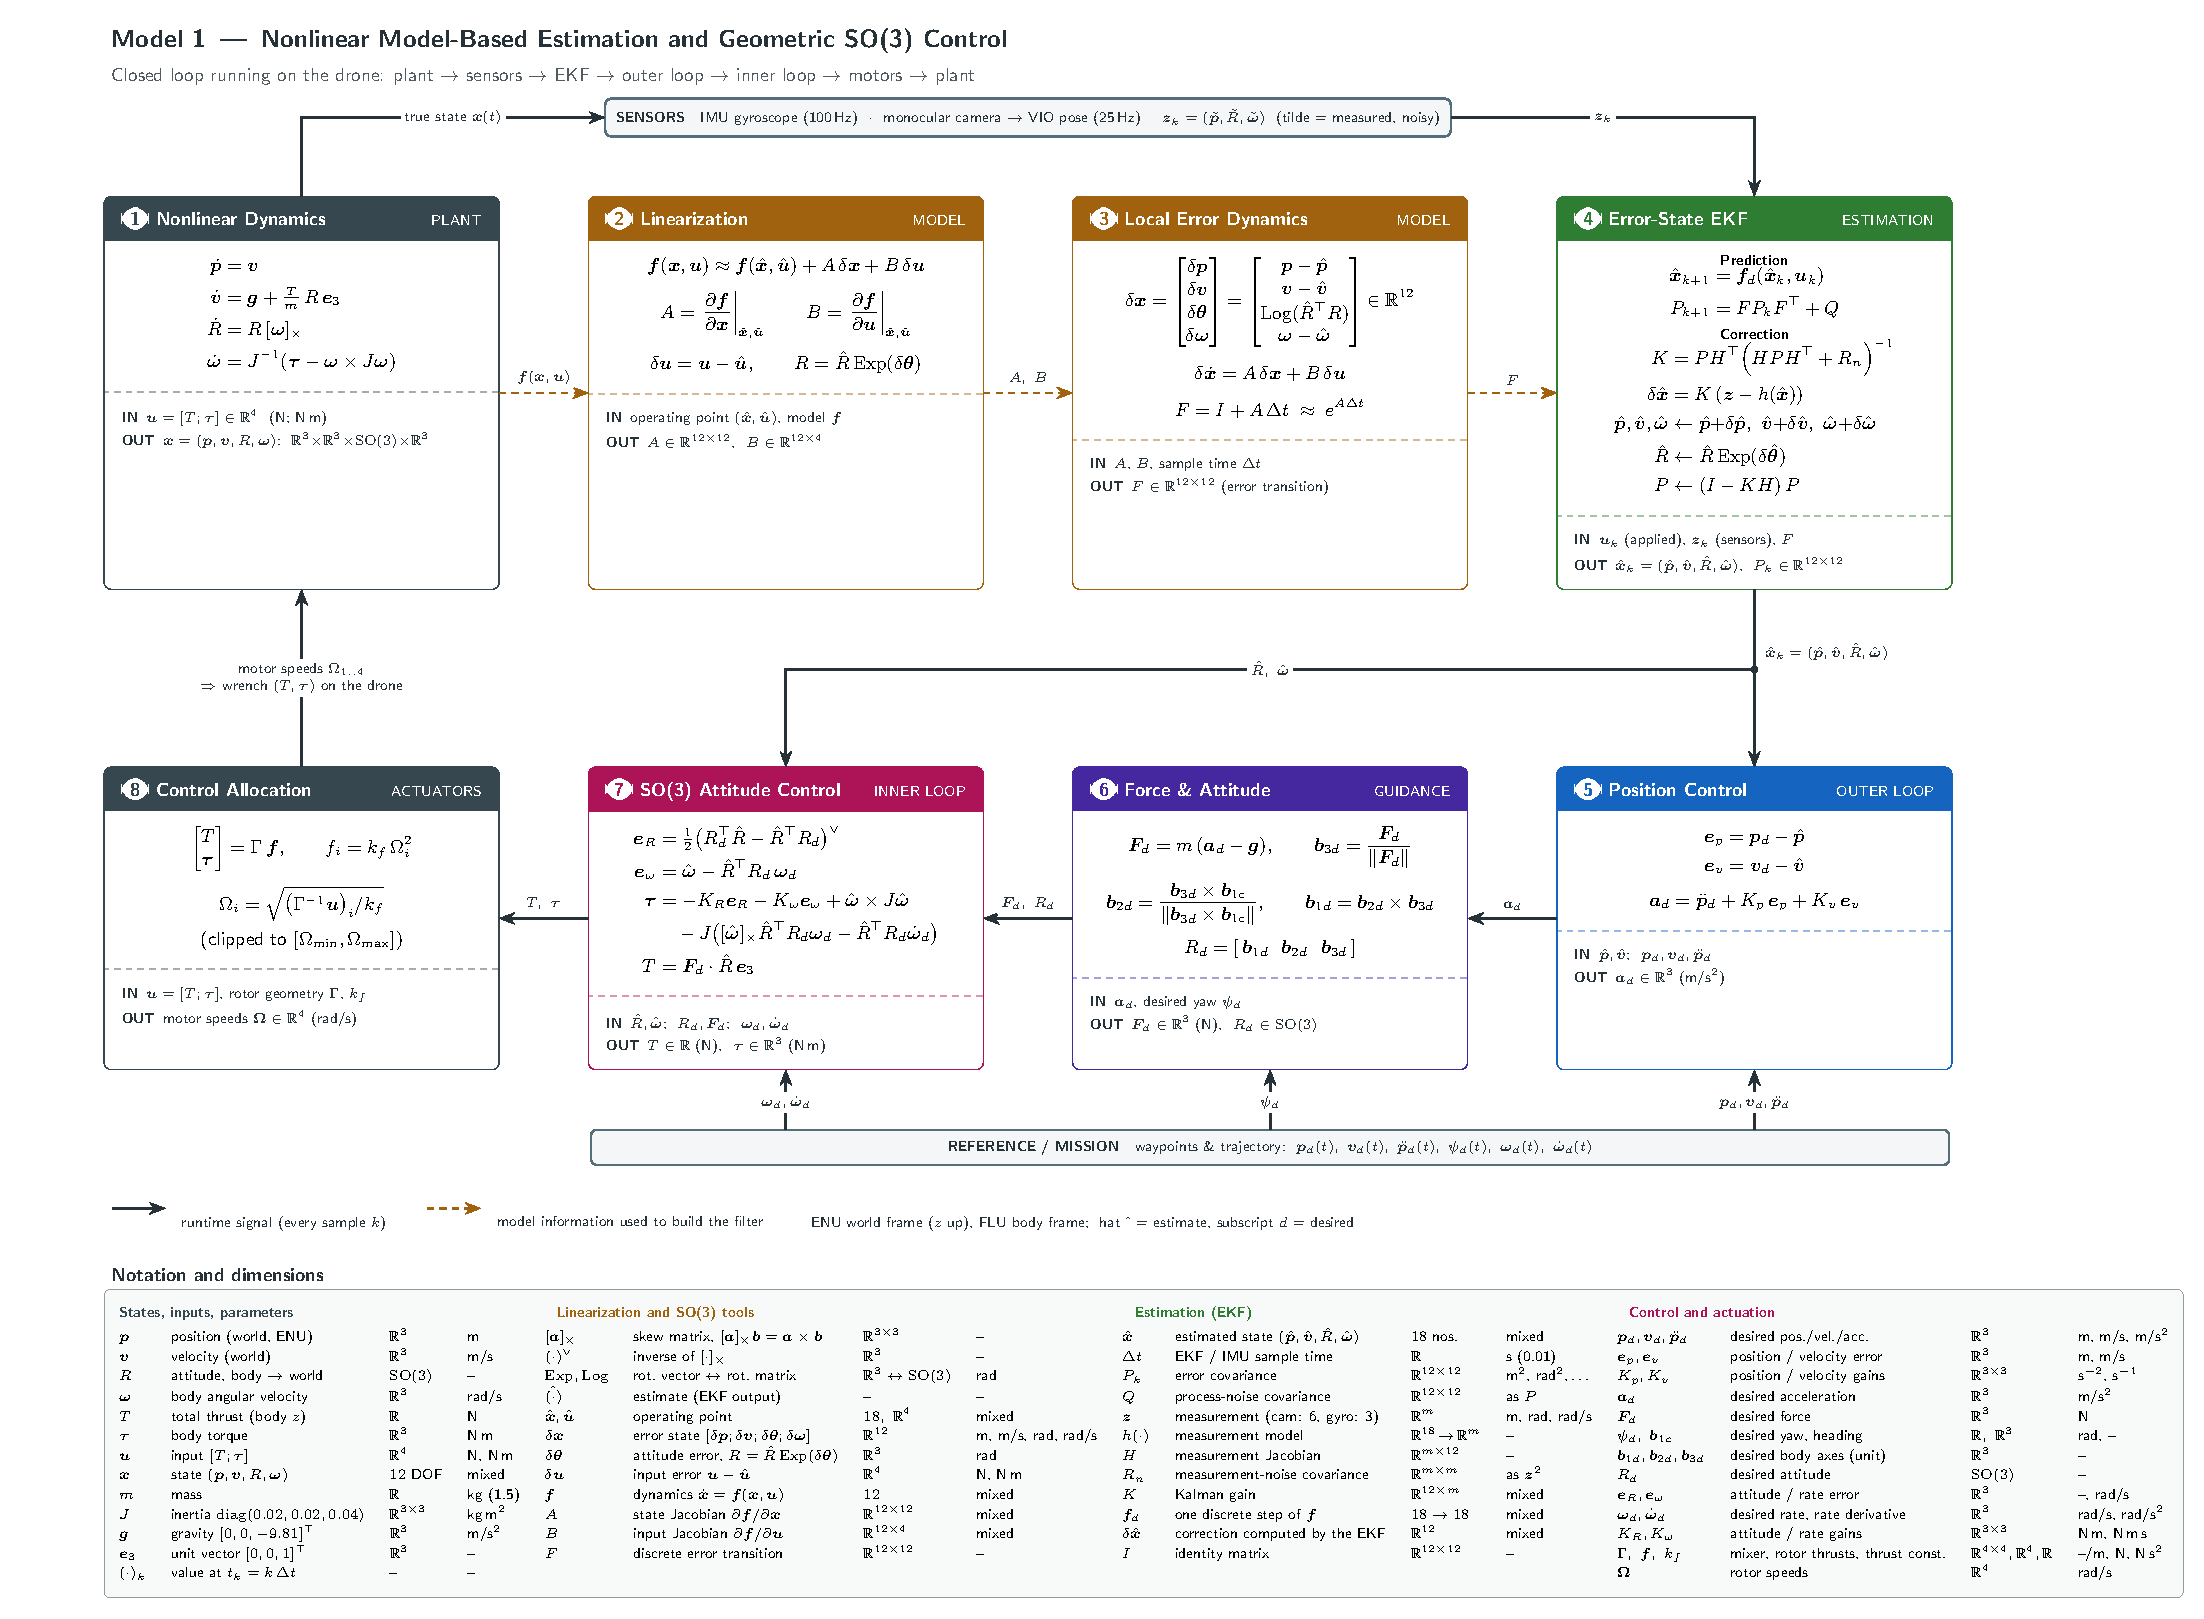
\includegraphics[width=\linewidth,height=16.4cm,keepaspectratio]{flow_model1.pdf}
  \caption{Model~1 equation flow: nonlinear model-based estimation and geometric $\SO$ control. The top row
  models and estimates the state, the bottom row controls it, and the left edge closes the loop through the
  motors. Dashed arrows carry model information (Jacobians) and solid arrows carry run-time signals.}
  \label{fig:flow1}
\end{figure}
\end{landscape}

\begin{figure}[p]
  \centering
  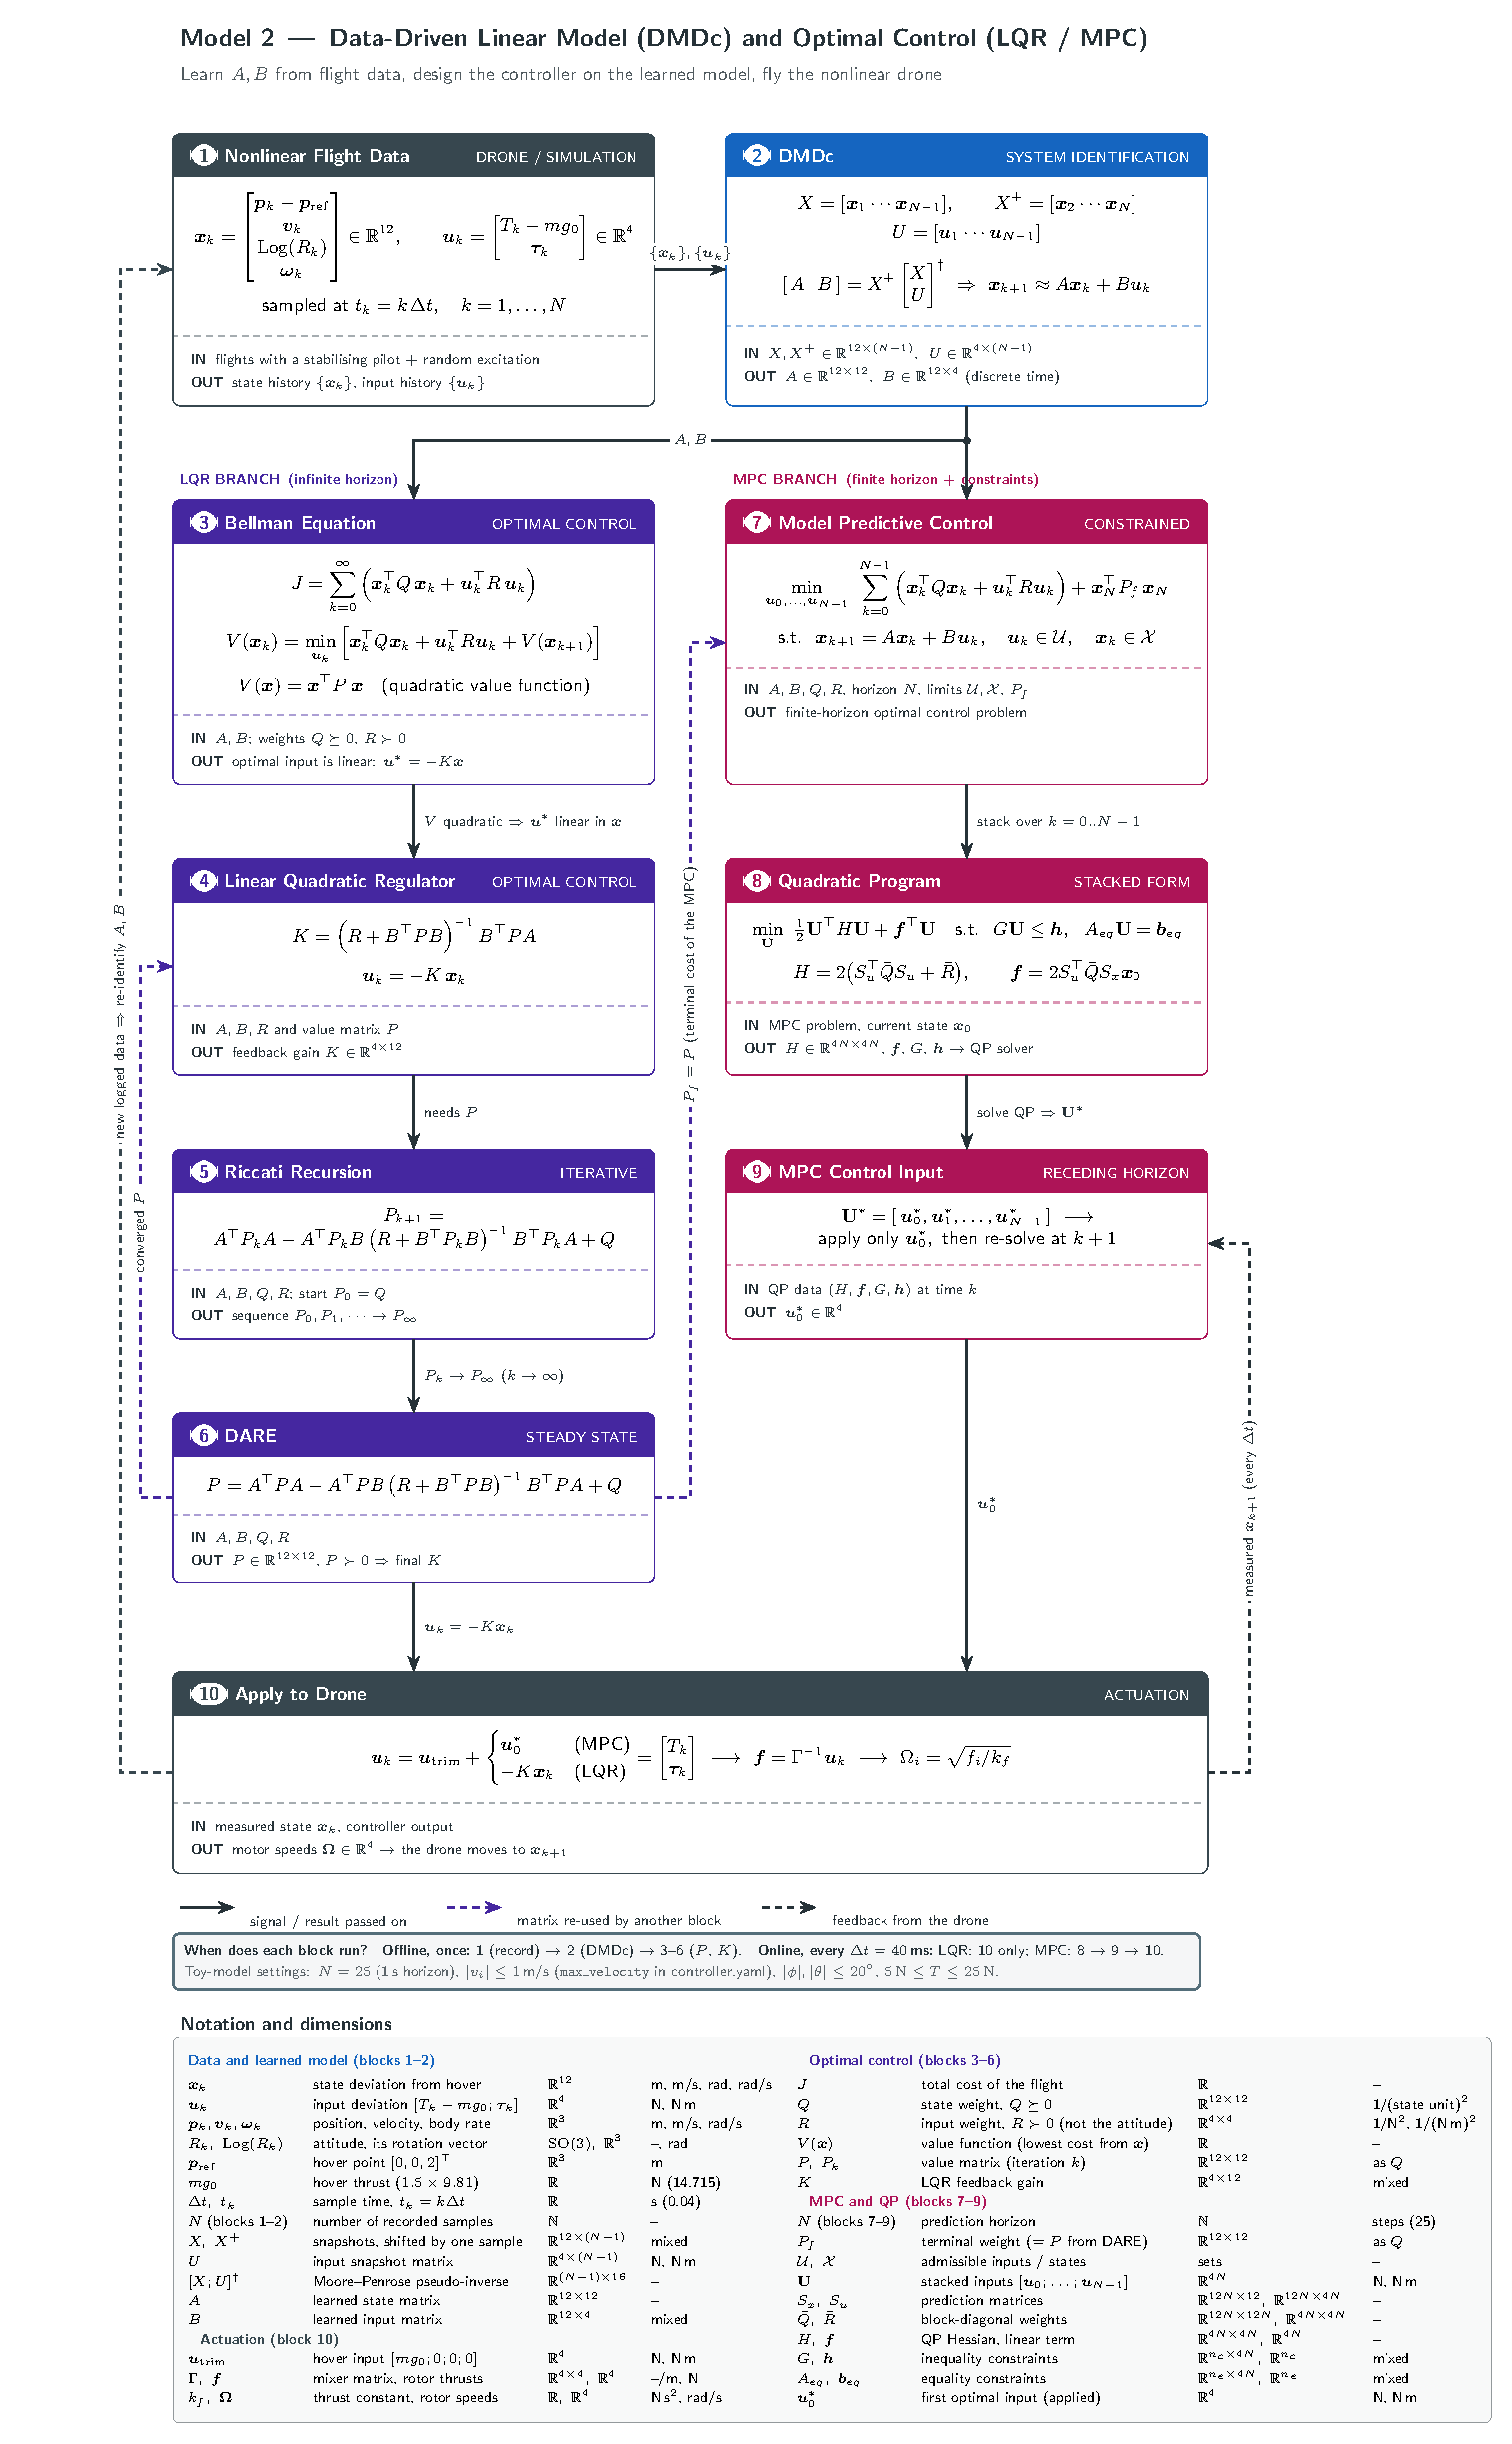
\includegraphics[width=\linewidth,height=0.93\textheight,keepaspectratio]{flow_model2.pdf}
  \caption{Model~2 equation flow: data-driven linear model (DMDc) followed by two optimal-control branches,
  LQR (left) and MPC (right), that meet when the command is applied to the drone.}
  \label{fig:flow2}
\end{figure}

% =====================================================================
\section[Model 1 --- Estimation and Geometric Control]{Model 1 --- Nonlinear Model-Based Estimation and Geometric Control}
\label{sec:model1}
% =====================================================================

Model~1 is the loop that actually flies the drone. It starts from physics (block~1). It builds the
small-error linear model that an estimator needs (blocks 2--3) and estimates the state from the sensors (block~4).
Finally it computes the commands in two nested loops, position (blocks 5--6) and attitude (block~7), and turns them
into motor speeds (block~8).

% ---------------------------------------------------------------------
\subsection{Block 1 --- Physical system and nonlinear dynamics}
\label{sec:m1b1}
% ---------------------------------------------------------------------

The drone is modelled as a single rigid body with mass $m$ and inertia $J$, pushed by a thrust $T$ along its own
$z$-axis and twisted by a torque $\vtau$. Its state is position, velocity, attitude and angular velocity.

\begin{eqbox}{cPlant}{Equations M1.1 -- M1.4 \quad Rigid-body dynamics of the quadrotor}
\begin{align}
  \dot{\vp} &= \vv \tag{M1.1}\label{eq:m1.1}\\
  \dot{\vv} &= \vg + \frac{T}{m}\,R\,\ve_3 \tag{M1.2}\label{eq:m1.2}\\
  \dot{R}   &= R\,\skw{\vw} \tag{M1.3}\label{eq:m1.3}\\
  \dot{\vw} &= J^{-1}\big(\vtau - \vw\times J\vw\big) \tag{M1.4}\label{eq:m1.4}
\end{align}
Compactly $\dot{\vx}=\vf(\vx,\vu)$ with state $\vx=(\vp,\vv,R,\vw)$ and input $\vu=[T;\vtau]$.
\end{eqbox}

\begin{dimtable}
\vp,\ \dot{\vp} & position and its rate (world frame) & \R^3 & m, m/s\\
\vv,\ \dot{\vv} & velocity and acceleration (world frame) & \R^3 & m/s, m/s$^2$\\
R,\ \dot R & attitude and its rate & \R^{3\times3} & --, 1/s\\
\vw,\ \dot{\vw} & body angular velocity and acceleration & \R^3 & rad/s, rad/s$^2$\\
T & total thrust & \R & N\\
\vtau & body torque & \R^3 & N\,m\\
\ve_3 & unit vector $[0,0,1]^\top$ & \R^3 & --\\
\vx & state (stored as 18 numbers, 12 degrees of freedom) & \R^3{\times}\R^3{\times}\SO{\times}\R^3 & mixed\\
\vu & input & \R^4 & N, N\,m\\
\end{dimtable}

\subsubsection*{Derivation}

\textbf{(M1.1) Kinematics.} Velocity is by definition the time derivative of position: $\vv=\frac{d\vp}{dt}$.

\textbf{(M1.2) Newton's second law.} In the inertial (world) frame, $m\dot{\vv}=\sum\vF$. Two forces act:
\begin{itemize}
  \item gravity, $m\vg$;
  \item rotor thrust. In the body frame it is $T\ve_3$ (straight ``up'' out of the propeller discs). Rotating it into
        the world frame gives $R\,T\ve_3=T\vb_3$.
\end{itemize}
Hence $m\dot{\vv}=m\vg+T R\ve_3$. Dividing by $m$ gives \eqref{eq:m1.2}. Air drag and wind are neglected in the
model. In the toy simulation they enter as an unknown disturbance, which is exactly what the controller must reject.

\textbf{(M1.3) Attitude kinematics.} Differentiate the constraint $R^\top R=I$:
\[
  \dot R^\top R+R^\top\dot R=0\quad\Longrightarrow\quad (R^\top\dot R)^\top=-R^\top\dot R .
\]
So $R^\top\dot R$ is skew-symmetric, which means it is the hat of some vector: $R^\top\dot R=\skw{\vw}$, i.e.\\
$\dot R=R\skw{\vw}$. Physically, a point fixed on the body at $\bm r^{\mathcal B}$ sits at $R\bm r^{\mathcal B}$ in the world.
Its velocity $\dot R\bm r^{\mathcal B}=R(\vw\times\bm r^{\mathcal B})$ is a rotation about the axis $\vw$, measured in the
body frame. That is exactly what a gyroscope bolted to the drone reports.

\textbf{(M1.4) Euler's rotation equation.} The angular momentum is $J\vw$ in the body frame and $\bm h=RJ\vw$ in the
world frame. Newton's law for rotation, $\dot{\bm h}=R\vtau$ (torque in world coordinates), together with \eqref{eq:m1.3}, gives
\[
  \frac{d}{dt}(RJ\vw)=\dot RJ\vw+RJ\dot{\vw}=R\big(\skw{\vw}J\vw+J\dot{\vw}\big)=R\vtau
  \ \Longrightarrow\ J\dot{\vw}+\vw\times J\vw=\vtau .
\]
The term $\vw\times J\vw$ is the \emph{gyroscopic} coupling. A body spinning about two axes at once produces a
rotation about the third axis without any torque.

\begin{toybox}[hover, tilt and gyroscopic coupling ($m=1.5$, $J=\diag(0.02,0.02,0.04)$)]
\textbf{Hover.} $R=I$, $\vw=0$, $T=mg_0=14.715$\,N, $\vtau=0$:
$\dot{\vv}=[0,0,-9.81]+\frac{14.715}{1.5}[0,0,1]=\bm 0$. The drone hangs still.

\textbf{10$^\circ$ roll with hover thrust.} $R\ve_3=[0,-\sin10^\circ,\cos10^\circ]^\top$, so
$\dot{\vv}=g_0[0,\,-\sin10^\circ,\,\cos10^\circ-1]^\top=[0,\,-1.7035,\,-0.1490]^\top$\,m/s$^2$.
It slides sideways and sinks slightly, because only $\cos10^\circ=98.5\%$ of the thrust still holds it up.

\textbf{Yaw rate.} $R=I$, $\vw=[0,0,0.5]^\top$: $\dot R=\skw{\vw}=\begin{bmatrix}0&-0.5&0\\0.5&0&0\\0&0&0\end{bmatrix}$,
so the body $x$-axis starts to turn towards $+y$ at 0.5\,rad/s.

\textbf{Gyroscopic coupling.} $\vw=[1,0,1]^\top$, $\vtau=0$: $J\vw=[0.02,0,0.04]^\top$,
$\vw\times J\vw=[0,\,-0.02,\,0]^\top$, so $\dot{\vw}=J^{-1}[0,0.02,0]^\top=[0,\,1,\,0]^\top$\,rad/s$^2$.
\end{toybox}

\begin{projbox}
These four lines are ``the real drone''. In our set-up they are solved by Gazebo for the Iris quadrotor, while
ArduPilot SITL plays the flight computer. Our ROS~2 node never integrates them. It \emph{reads} their result on
\code{/ap/v1/pose/filtered} (position $\vp$ and orientation quaternion $\to R$) and
\code{/ap/v1/twist/filtered} ($\vv$, $\vw$). Everything else in this document either predicts this motion
(the EKF), steers it (the controller), or learns it from data (Model~2).
\end{projbox}

\begin{codebox}
\intoy \code{model1\_nonlinear\_ekf\_so3/step1\_nonlinear\_dynamics.m}, \code{lib/quad\_dynamics.m}
(RK4 integration in \code{lib/rk4\_step.m}). A 0.01\,N\,m roll-torque pulse of 0.1\,s already makes the open-loop
drone drift 2.1\,m in 4\,s (\code{figures/step1\_open\_loop.png}).
\end{codebox}

% ---------------------------------------------------------------------
\subsection{Block 2 --- Linearization: Taylor expansion and Jacobians}
\label{sec:m1b2}
% ---------------------------------------------------------------------

\begin{eqbox}{cModel}{Equations M1.5 -- M1.6 \quad First-order Taylor expansion and Jacobians}
\begin{align}
  \vf(\vx,\vu) &\approx \vf(\hx,\hu) + A\,\delta\vx + B\,\delta\vu,\qquad \delta\vx\ \text{from \eqref{eq:dx}},\ \ \delta\vu=\vu-\hu \tag{M1.5}\label{eq:m1.5}\\
  A &= \left.\frac{\partial\vf}{\partial\vx}\right|_{\hx,\hu}\in\R^{12\times12},\qquad
  B = \left.\frac{\partial\vf}{\partial\vu}\right|_{\hx,\hu}\in\R^{12\times4} \tag{M1.6}\label{eq:m1.6}
\end{align}
\end{eqbox}

\begin{dimtable}
\hx,\ \hu & operating point (where we linearize) & \R^{18},\ \R^4 & mixed\\
\delta\vx & state error $[\vp-\hp;\ \vv-\hv;\ \Log(\hR^\top R);\ \vw-\hw]$ & \R^{12} & m, m/s, rad, rad/s\\
\delta\vu=\vu-\hu & input error $[\delta T;\delta\vtau]$ & \R^4 & N, N\,m\\
A & state Jacobian & \R^{12\times12} & mixed (1/s, m/s$^2$\dots)\\
B & input Jacobian & \R^{12\times4} & mixed (1/kg, 1/(kg\,m$^2$))\\
\end{dimtable}

\subsubsection*{Derivation of the Taylor expansion}

For a smooth vector function, Taylor's theorem in several variables states
\[
  \vf(\hx+\delta\vx,\hu+\delta\vu)=\vf(\hx,\hu)+\frac{\partial\vf}{\partial\vx}\delta\vx+\frac{\partial\vf}{\partial\vu}\delta\vu
  +\mathcal O\big(\|\delta\vx\|^2+\|\delta\vu\|^2\big).
\]
Dropping the second-order remainder gives \eqref{eq:m1.5}. Entry $(i,j)$ of $A$ is $\partial f_i/\partial x_j$, i.e.\\
how much the rate of state $i$ changes when state $j$ is nudged. Because $R$ lives on $\SO$, ``nudging'' the
attitude means $R=\hR\,\Exp(\delta\vth)$, so the attitude part of $\delta\vx$ has 3 entries, not 9.

\subsubsection*{Derivation of $A$ and $B$ for the drone}

Insert $\vp=\hp+\delta\vp$, $\vv=\hv+\delta\vv$, $R=\hR\Exp(\delta\vth)\approx\hR(I+\skw{\delta\vth})$, $\vw=\hw+\delta\vw$,
$T=\hat T+\delta T$, $\vtau=\hat{\vtau}+\delta\vtau$ into \eqref{eq:m1.1}--\eqref{eq:m1.4} and keep first-order terms.

\begin{itemize}
\item \textbf{Position:} $\delta\dot{\vp}=\delta\vv$.
\item \textbf{Velocity:}
  $\dot{\vv}\approx\vg+\frac{\hat T+\delta T}{m}\hR(I+\skw{\delta\vth})\ve_3$. Using
  $\skw{\delta\vth}\ve_3=\delta\vth\times\ve_3=-\skw{\ve_3}\delta\vth$ and dropping the product $\delta T\,\delta\vth$:
  \[\delta\dot{\vv}=-\frac{\hat T}{m}\hR\skw{\ve_3}\,\delta\vth+\frac{1}{m}\hR\ve_3\,\delta T .\]
\item \textbf{Attitude:} differentiate $R=\hR\Exp(\delta\vth)$ with $\dot R=R\skw{\vw}$ and $\dot{\hR}=\hR\skw{\hw}$. To first order,
  $\skw{\delta\dot{\vth}}=\skw{\delta\vw}+\skw{\delta\vth}\skw{\hw}-\skw{\hw}\skw{\delta\vth}=\skw{\delta\vw}-\skw{\hw\times\delta\vth}$, so
  \[\delta\dot{\vth}=-\skw{\hw}\,\delta\vth+\delta\vw .\]
\item \textbf{Angular rate:} $\frac{\partial}{\partial\vw}(\vw\times J\vw)=\skw{\vw}J-\skw{J\vw}$, hence
  \[\delta\dot{\vw}=J^{-1}\big(\skw{J\hw}-\skw{\hw}J\big)\delta\vw+J^{-1}\delta\vtau .\]
\end{itemize}

Stacking the four rows gives
\begin{equation}
\label{eq:AB}
A=\begin{bmatrix}
0&I&0&0\\
0&0&-\frac{\hat T}{m}\hR\skw{\ve_3}&0\\
0&0&-\skw{\hw}&I\\
0&0&0&J^{-1}\big(\skw{J\hw}-\skw{\hw}J\big)
\end{bmatrix},\qquad
B=\begin{bmatrix}0&0\\ \frac1m\hR\ve_3&0\\ 0&0\\ 0&J^{-1}\end{bmatrix}.
\end{equation}

At hover ($\hR=I$, $\hw=0$, $\hat T=mg_0$) the key blocks become
\[
-g_0\skw{\ve_3}=\begin{bmatrix}0&9.81&0\\-9.81&0&0\\0&0&0\end{bmatrix},\qquad
\tfrac1m\ve_3=\begin{bmatrix}0\\0\\0.667\end{bmatrix},\qquad
J^{-1}=\diag(50,50,25).
\]
Read row by row: a pitch error $\delta\theta_y$ accelerates the drone along $+x$ at $9.81\,\delta\theta_y$\,m/s$^2$.
A roll error $\delta\theta_x$ accelerates it along $-y$. Extra thrust only changes vertical acceleration. Torque changes
angular acceleration with gain $1/J$.

\begin{toybox}[how good is ``first order''?]
Pitch the hovering drone by $\theta$. The linear model predicts $\dot v_x=g_0\theta$; the truth is $g_0\sin\theta$.
\begin{center}\small
\begin{tabular}{rrrr}
\toprule
$\theta$ [deg] & linear $g_0\theta$ [m/s$^2$] & true $g_0\sin\theta$ [m/s$^2$] & error\\
\midrule
1.00 & 0.1712 & 0.1712 & 0.005\%\\
2.87 (0.05 rad) & 0.4905 & 0.4903 & 0.04\%\\
10.00 & 1.7122 & 1.7035 & 0.51\%\\
20.00 & 3.4243 & 3.3552 & 2.06\%\\
28.65 (0.5 rad) & 4.9054 & 4.7035 & 4.29\%\\
\bottomrule
\end{tabular}
\end{center}
The analytic Jacobians \eqref{eq:AB} were also checked against numerical differentiation of the true flow at a
tilted, spinning, accelerating state. The largest difference is $2.3\times10^{-8}$ for $A$ and $8.4\times10^{-7}$ for $B$.
\end{toybox}

\begin{projbox}
Linearization is the ``zoom-in'' trick. Near any flight condition the complicated drone behaves like a simple
linear system, and linear systems are easy to reason about. Our EKF uses $A$ to answer one question every 10\,ms:
\emph{how fast does my uncertainty grow if I trust only the physics?} The table shows the trick is excellent for
the gentle tilts of normal flight (below 10$^\circ$, under 0.5\% error). That is why both the EKF and Model~2
can rely on it.
\end{projbox}

\begin{codebox}
\intoy \code{step2\_taylor\_jacobian.m}, \code{lib/quad\_jacobians.m}; figure \code{step2\_taylor\_accuracy.png}.
\end{codebox}

% ---------------------------------------------------------------------
\subsection{Block 3 --- Local error dynamics}
\label{sec:m1b3}
% ---------------------------------------------------------------------

\begin{eqbox}{cModel}{Equations M1.7 -- M1.9 \quad Linear dynamics of the estimation error}
\begin{align}
  \delta\vx &= \big[\vp-\hp;\ \vv-\hv;\ \Log(\hR^\top R);\ \vw-\hw\big] \tag{M1.7}\label{eq:m1.7}\\
  \delta\dot{\vx} &= A\,\delta\vx + B\,\delta\vu \tag{M1.8}\label{eq:m1.8}\\
  \delta\vx_{k+1} &= F\,\delta\vx_k + G\,\delta\vu_k,\qquad F=e^{A\Delta t}\approx I+A\Delta t,\quad G\approx B\Delta t \tag{M1.9}\label{eq:m1.9}
\end{align}
\end{eqbox}

\begin{dimtable}
\delta\vx & error between true and estimated (or nominal) state & \R^{12} & mixed\\
F & discrete error-transition matrix & \R^{12\times12} & --\\
G & discrete input matrix & \R^{12\times4} & mixed\\
\Delta t & sample time & \R & s (0.01)\\
\end{dimtable}

\subsubsection*{Derivation}

The true state obeys $\dot{\vx}=\vf(\vx,\vu)$ and the reference (estimated) state obeys the same model,
$\dot{\hx}=\vf(\hx,\hu)$. Subtracting, and using \eqref{eq:m1.5},
\[
  \delta\dot{\vx}=\vf(\vx,\vu)-\vf(\hx,\hu)\approx\big[\vf(\hx,\hu)+A\delta\vx+B\delta\vu\big]-\vf(\hx,\hu)=A\delta\vx+B\delta\vu .
\]
The large nonlinear parts cancel and only the small, linear error remains. Over one sample, with $A$ and $\delta\vu$
held constant, the solution of this linear ODE is
$\delta\vx(t_k+\Delta t)=e^{A\Delta t}\delta\vx(t_k)+\int_0^{\Delta t}e^{A s}\,ds\,B\,\delta\vu_k$.
The series $e^{A\Delta t}=I+A\Delta t+\frac12(A\Delta t)^2+\dots$ truncated after the linear term gives
\eqref{eq:m1.9}. This is exactly the forward-Euler step.

\textbf{Why the error grows without feedback.} At hover every eigenvalue of $A$ is zero ($A$ is nilpotent).
The chain $\delta\vw\to\delta\vth\to\delta\vv\to\delta\vp$ is four integrators in series, so a constant rate error
grows into a position error proportional to $t^3$. The drone is \emph{open-loop unstable}. That is why it needs both a
good estimate (block~4) and feedback (blocks 5--7).

\begin{toybox}[propagate an error for 2 s]
Extra thrust $\delta T=0.5$\,N at hover. Only row 6 of $B$ is non-zero, so
$\delta v_z(t)=\frac{\delta T}{m}t=\frac{0.5}{1.5}\cdot2=0.667$\,m/s. The linear model gives 0.6667 and the nonlinear
truth 0.6543.

Initial error $2^\circ$ roll, 10\,cm, 0.2\,rad/s yaw rate: after 2\,s the linear prediction differs from the truth by
2.6\%. With a $30^\circ$ initial roll the difference is 26\%. The linear model is \emph{local}.

With $\Delta t=0.01$\,s, $\max|F-e^{A\Delta t}|=4.9\times10^{-4}$, the size of the neglected
$\tfrac12(A\Delta t)^2$ term.
\end{toybox}

\begin{projbox}
The EKF never tries to describe the whole flight with a linear model. It only describes the
\emph{small difference} between what it believes and what is true, and that difference \emph{is} small, because the
camera and IMU keep correcting it. This is the reason for the name \emph{error-state} filter.
\end{projbox}

\begin{codebox}
\intoy \code{step3\_local\_error\_dynamics.m}; figure \code{step3\_error\_dynamics.png}.
\end{codebox}

% ---------------------------------------------------------------------
\subsection{Block 4 --- State estimation: error-state EKF}
\label{sec:m1b4}
% ---------------------------------------------------------------------

\begin{keybox}
\textbf{The idea before the maths.} The filter repeats two steps forever.
\begin{enumerate}[leftmargin=*]
  \item \textbf{Predict.} ``I know how I pushed the drone, so the physics tells me where it should be now.''
        The guess moves forward, and because physics is never perfect, the uncertainty \emph{grows}.
  \item \textbf{Correct.} ``A sensor reading has arrived. How surprised am I?'' The guess is pulled towards the
        measurement, by an amount that depends on whom we trust more, and the uncertainty \emph{shrinks}.
\end{enumerate}
The filter stores two things: the \textbf{estimate} $\hx_k=(\hp,\hv,\hR,\hw)$ (its best guess) and the
\textbf{covariance} $P_k$ (how unsure it is about each of the 12 error directions of \eqref{eq:dx}).
\end{keybox}

\textbf{Assumptions about noise.} The real drone follows the model only approximately. Each step it is pushed by
a small unknown random error $\bm w_k$ (wind, model mistakes) with covariance $Q$. Every sensor reads the true
value plus a random error $\bm v_k$ with covariance $R_n$:
\[
  \vx_{k+1}=\vf_d(\vx_k,\vu_k)\ \text{plus a random error }\bm w_k\sim\mathcal N(0,Q),\qquad
  \vz_k=h(\vx_k)+\bm v_k,\quad \bm v_k\sim\mathcal N(0,R_n).
\]
Here $\vf_d$ is one simulation step (RK4) of \eqref{eq:m1.1}--\eqref{eq:m1.4}, and $\mathcal N(0,Q)$ means ``Gaussian
with mean zero and covariance $Q$''. The errors are added in the 12 error directions, so for the attitude
``adding'' means a small rotation, as in \eqref{eq:correct}.

\begin{eqbox}{cEst}{Equations M1.10 -- M1.14 \quad Error-state EKF}
\textbf{Time update (prediction)}
\begin{align}
  \hx_{k+1} &= \vf_d(\hx_k,\vu_k) \tag{M1.10}\label{eq:m1.10}\\
  P_{k+1}   &= F P_k F^\top + Q \tag{M1.11}\label{eq:m1.11}
\end{align}
\textbf{Measurement update (correction)}
\begin{align}
  K   &= P H^\top\big(HPH^\top+R_n\big)^{-1} \tag{M1.12}\label{eq:m1.12}\\
  \delta\hat{\vx} &= K\,\vr,\qquad \vr=\vz-h(\hx)\ \ \text{(innovation)},\qquad
  \text{then correct } \hx \text{ by } \delta\hat{\vx} \text{ using \eqref{eq:correct}} \tag{M1.13}\label{eq:m1.13}\\
  P   &\leftarrow (I-KH)\,P \tag{M1.14}\label{eq:m1.14}
\end{align}
Written out, the correction in (M1.13) is
$\hp\leftarrow\hp+\delta\hat{\vp}$, $\hv\leftarrow\hv+\delta\hat{\vv}$, $\hR\leftarrow\hR\,\Exp(\delta\hat{\vth})$,
$\hw\leftarrow\hw+\delta\hat{\vw}$.
\end{eqbox}

\begin{dimtable}
\hx_k & estimated state $(\hp,\hv,\hR,\hw)$ & \R^{18} & mixed\\
P_k & error covariance & \R^{12\times12} & m$^2$, (m/s)$^2$, rad$^2$, \dots\\
Q & process-noise covariance per step (wind, model error) & \R^{12\times12} & as $P$\\
\vz & measurement (camera pose: $m=6$, gyro: $m=3$) & \R^m & m, rad, rad/s\\
h(\cdot) & measurement model & \R^{18}\to\R^m & --\\
H=\partial h/\partial\delta\vx & measurement Jacobian & \R^{m\times12} & --\\
R_n & measurement-noise covariance & \R^{m\times m} & m$^2$, rad$^2$, \dots\\
K & Kalman gain & \R^{12\times m} & mixed\\
\vr=\vz-h(\hx) & innovation: measured minus expected (``surprise'') & \R^m & as $\vz$\\
\delta\hat{\vx} & correction computed from the innovation & \R^{12} & mixed\\
\end{dimtable}

\subsubsection*{Derivation}

\textbf{(M1.10) Mean prediction.} The truth is the estimate corrected by an unknown error $\delta\vx_k$ whose
average is zero (a good estimate is not biased to one side). By the linearization of block~3, one step later the
truth is $\vf_d(\hx_k,\vu_k)$ corrected by $F\delta\vx_k$. Since $\delta\vx_k$ averages to zero, so does $F\delta\vx_k$,
and the best guess of the next state is simply $\vf_d(\hx_k,\vu_k)$. The full nonlinear model is used for the guess
itself. The linear model is only needed for the uncertainty.

\textbf{(M1.11) Covariance prediction.} From \eqref{eq:m1.9} plus noise, $\delta\vx_{k+1}=F\delta\vx_k+\bm w_k$. Then
\[
  P_{k+1}=\mathbb E[\delta\vx_{k+1}\delta\vx_{k+1}^\top]
  =F\,\mathbb E[\delta\vx_k\delta\vx_k^\top]F^\top+\mathbb E[\bm w_k\bm w_k^\top]
  =FP_kF^\top+Q,
\]
because the noise is independent of the current error, so the cross terms vanish. Uncertainty is stretched by
the dynamics ($F\cdot F^\top$) and inflated by the noise ($+Q$).

\textbf{(M1.12) Kalman gain.} Linearize the measurement: the innovation $\vr=\vz-h(\hx)\approx H\delta\vx+\bm v$
(``what I see minus what I expected = my error seen through the sensor, plus sensor noise'').
We correct the error estimate by a linear rule $\delta\hat{\vx}=K\vr$. The error after the correction is
$\delta\vx^+=\delta\vx-K(H\delta\vx+\bm v)=(I-KH)\delta\vx-K\bm v$, whose covariance is
\begin{equation}
\label{eq:joseph}
  P^+=(I-KH)P(I-KH)^\top+KR_nK^\top \qquad\text{(Joseph form, valid for any $K$).}
\end{equation}
The best $K$ minimises the total variance $\tr P^+$. Using $\frac{\partial}{\partial K}\tr(KMK^\top)=2KM$ for
symmetric $M$ and $\frac{\partial}{\partial K}\tr(KN)=N^\top$:
\[
  \frac{\partial\,\tr P^+}{\partial K}=-2PH^\top+2K\big(HPH^\top+R_n\big)=0
  \ \Longrightarrow\ K=PH^\top\underbrace{\big(HPH^\top+R_n\big)}_{S\ \text{(innovation covariance)}}{}^{-1}.
\]

\textbf{(M1.13) State update.} The best estimate of the error is $\delta\hat{\vx}=K\vr$. It is applied to the
estimate with the correction rule \eqref{eq:correct}: positions, velocities and rates are added, and the attitude
is rotated, $\hR\leftarrow\hR\Exp(\delta\hat{\vth})$, so $\hR$ stays a valid rotation matrix. The error has now been
absorbed into the estimate, so the filter starts the next step believing its error is zero on average again.

\textbf{(M1.14) Covariance update.} Expand \eqref{eq:joseph} and use $KS=PH^\top$:
$P^+=P-KHP-PH^\top K^\top+KSK^\top=P-KHP-PH^\top K^\top+PH^\top K^\top=(I-KH)P$.
The toy code uses this short form and re-symmetrises $P$ after every step.

\subsubsection*{Our measurement models}

\begin{center}\small
\begin{tabular}{@{}llll@{}}
\toprule
Sensor (rate) & innovation $\vr$ & $H$ & noise $\sqrt{\diag R_n}$\\
\midrule
Gyroscope (100\,Hz) & $\tilde{\vw}-\hw$ & $[\,0\ \ 0\ \ 0\ \ I\,]$ & 0.01\,rad/s\\
Camera / VIO pose (25\,Hz) & $\begin{bmatrix}\tilde{\vp}-\hp\\ \Log(\hR^\top\tilde R)\end{bmatrix}$ &
  $\begin{bmatrix}I&0&0&0\\0&0&I&0\end{bmatrix}$ & 0.05\,m, 0.02\,rad\\
\bottomrule
\end{tabular}
\end{center}
Each block of $H$ is $3\times3$, and the columns follow $[\delta\vp,\delta\vv,\delta\vth,\delta\vw]$. Velocity is
\emph{never measured}. The filter infers it from how the measured position changes and from the physics in $F$.

\begin{toybox}[one predict + one correct, altitude only]
Prior: altitude $\hat z_k=10$\,m, variance $P_k=3.5$\,m$^2$. Commanded climb 0.5\,m/s for $\Delta t=1$\,s, $F=1$, $Q=0.5$:
\[\hat z^-=10+0.5=10.5\ \text{m},\qquad P^-=1\cdot3.5\cdot1+0.5=4.0\ \text{m}^2.\]
GPS reads $z=12.5$\,m with $R_n=1$\,m$^2$, $H=1$:
\[K=\frac{4}{4+1}=0.8,\quad \hat z^+=10.5+0.8\,(12.5-10.5)=12.1\ \text{m},\quad P^+=(1-0.8)\cdot4=0.8\ \text{m}^2.\]
The GPS is four times more trustworthy than the prediction ($P^-/R_n=4$), so the estimate moves 80\% of the way
towards it, and the variance shrinks from 4.0 to 0.8.

\textbf{Full 12-state filter} (20\,s helix flight, gusts, noisy sensors, wrong initial guess):
\begin{center}\small
\begin{tabular}{lrl}
\toprule
quantity & RMSE after 2\,s & for comparison\\
\midrule
position & 2.55\,cm & raw camera: 8.55\,cm\\
velocity (never measured) & 3.9\,cm/s & --\\
attitude & 0.20$^\circ$ & camera noise: 1.15$^\circ$\\
body rate & 0.0025\,rad/s & gyro noise: 0.01\,rad/s\\
\bottomrule
\end{tabular}
\end{center}
In 99\% of the samples all 12 errors lie inside the $\pm3\sigma$ band predicted by $P_k$, so the filter is
\emph{consistent}: it knows how uncertain it is.
\end{toybox}

\begin{figure}[h]
  \centering
  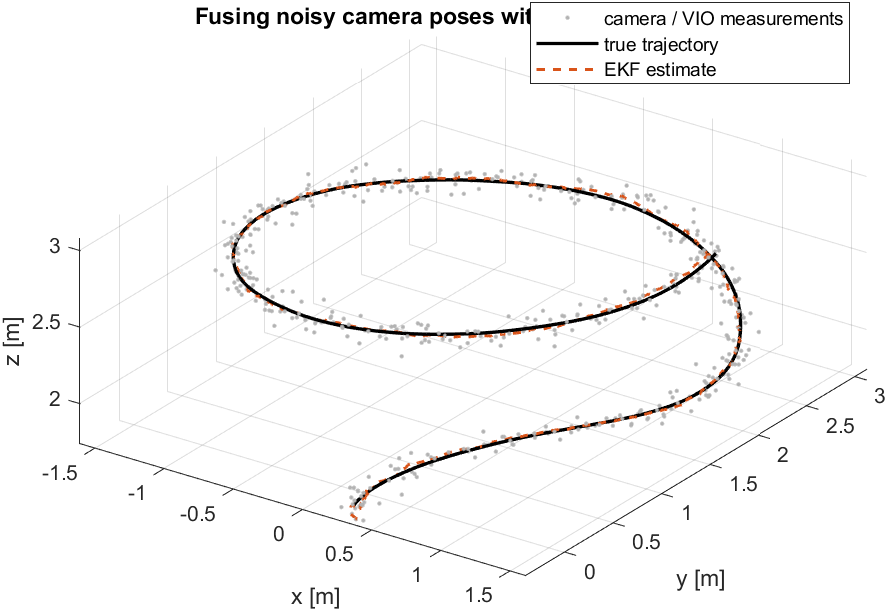
\includegraphics[width=0.49\linewidth]{step4_ekf_trajectory.png}\hfill
  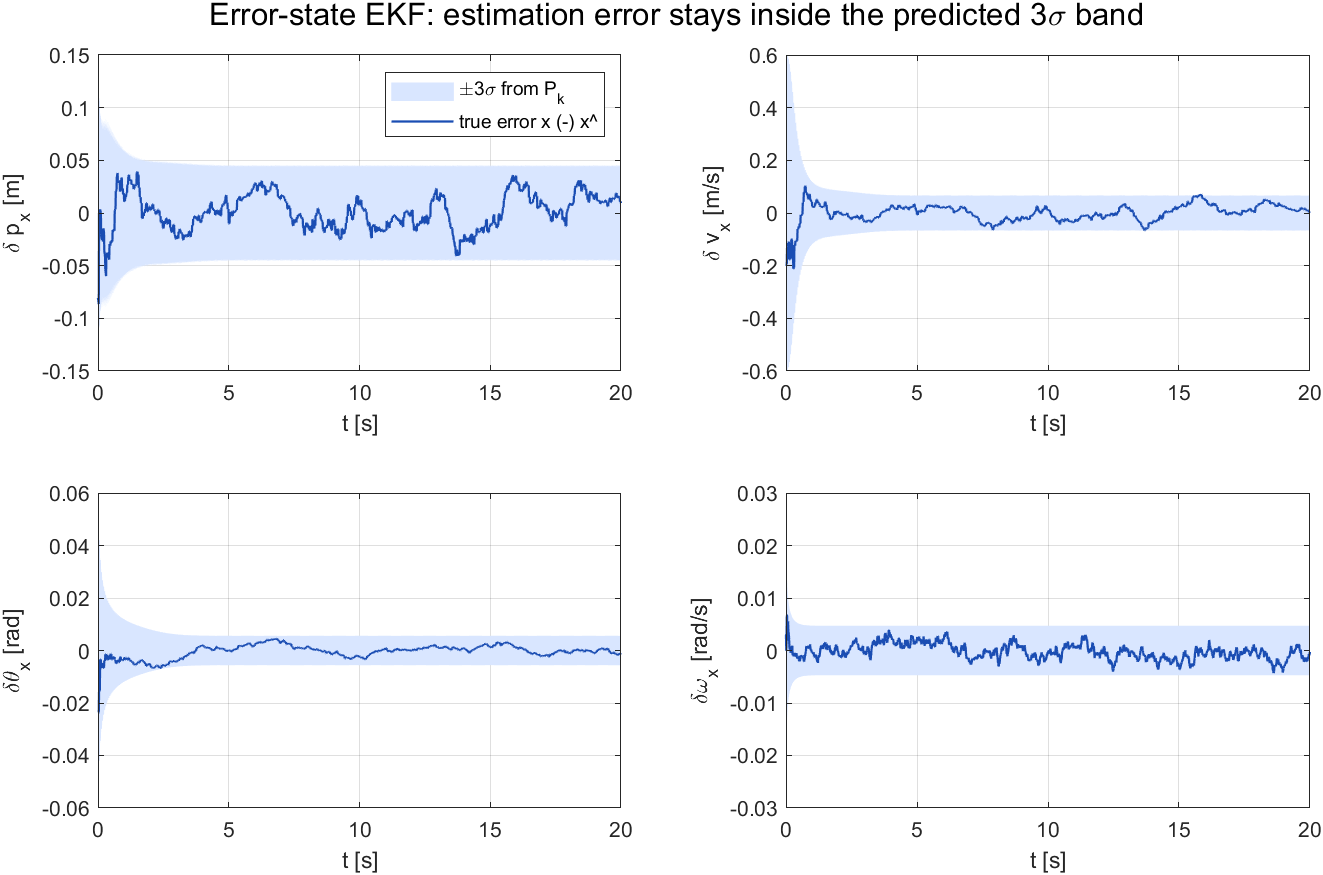
\includegraphics[width=0.49\linewidth]{step4_ekf_errors.png}
  \caption{Toy model, Model~1 step~4. Left: noisy camera positions (grey), truth (black) and EKF estimate.
  Right: estimation errors stay inside the $\pm3\sigma$ band computed from $P_k$.}
  \label{fig:m1-ekf}
\end{figure}

\begin{projbox}[this is the ``VIO'' of our title]
A monocular camera alone cannot tell scale (a small room close up looks like a big room far away), and an IMU
alone drifts within seconds. The EKF is the referee that fuses them. Between camera frames it predicts with the
physics and the gyro. When a frame arrives, the visual-odometry pose corrects the prediction, and $K$ decides how much
to trust each source. Its output $\hx$ (position, velocity, attitude, rate) is the only thing the controller ever
sees. In the current SITL set-up ArduPilot's own EKF3 produces \code{/ap/v1/*/filtered}. Our VIO pipeline supplies
the camera measurement $\vz_{\text{cam}}$ to exactly this structure.
\end{projbox}

\begin{codebox}
\intoy \code{step4\_error\_state\_ekf.m}, \code{lib/ekf\_predict.m}, \code{lib/ekf\_update.m}.
\end{codebox}

% ---------------------------------------------------------------------
\subsection{Block 5 --- Position control (outer loop)}
\label{sec:m1b5}
% ---------------------------------------------------------------------

\begin{eqbox}{cOuter}{Equations M1.15 -- M1.16 \quad Tracking errors and desired acceleration}
\begin{align}
  \ve_p=\vp_d-\hp,\qquad \ve_v&=\vv_d-\hv \tag{M1.15}\label{eq:m1.15}\\
  \va_d&=\ddot{\vp}_d+K_p\,\ve_p+K_v\,\ve_v \tag{M1.16}\label{eq:m1.16}
\end{align}
\end{eqbox}

\begin{dimtable}
\vp_d,\ \vv_d,\ \ddot{\vp}_d & desired position, velocity, acceleration & \R^3 & m, m/s, m/s$^2$\\
\ve_p,\ \ve_v & position and velocity error & \R^3 & m, m/s\\
K_p & position gain (diagonal, positive) & \R^{3\times3} & 1/s$^2$\\
K_v & velocity gain (diagonal, positive) & \R^{3\times3} & 1/s\\
\va_d & desired acceleration & \R^3 & m/s$^2$\\
\end{dimtable}

\subsubsection*{Derivation}

Suppose the inner loops achieve the commanded acceleration exactly, $\ddot{\vp}=\va_d$. Then the position error
obeys
\[
  \ddot{\ve}_p=\ddot{\vp}_d-\ddot{\vp}=\ddot{\vp}_d-\va_d=-K_p\ve_p-K_v\dot{\ve}_p
  \quad\Longrightarrow\quad \ddot{\ve}_p+K_v\dot{\ve}_p+K_p\ve_p=\bm0 .
\]
With diagonal gains, each axis is a mass--spring--damper with characteristic polynomial $s^2+k_vs+k_p$.
Both roots have negative real part if and only if $k_p,k_v>0$, so the error decays to zero. Matching with
$s^2+2\zeta\omega_ns+\omega_n^2$:
\[
  \omega_n=\sqrt{k_p},\qquad \zeta=\frac{k_v}{2\sqrt{k_p}},\qquad t_{2\%}\approx\frac{4}{\zeta\omega_n}.
\]
The feed-forward $\ddot{\vp}_d$ supplies the acceleration a perfect pilot would need. The feedback terms only fix what
is left over.

\begin{center}\small
\begin{tabular}{@{}lrrrrr@{}}
\toprule
axis & $k_p$ & $k_v$ & $\omega_n$ [rad/s] & $\zeta$ & $t_{2\%}$ [s]\\
\midrule
$x,\ y$ & 1.5 & 1.2 & 1.225 & 0.490 & 6.7\\
$z$ & 2.0 & 1.5 & 1.414 & 0.530 & 5.3\\
\bottomrule
\end{tabular}
\end{center}
These are our \code{controller.yaml} gains: gentle, slightly under-damped, a little overshoot, settling in about 6\,s.

\begin{toybox}[50 cm low and climbing]
Setpoint $\vp_d=[0,0,2]$\,m (the \code{controller.yaml} hover point), $\vv_d=\ddot{\vp}_d=\bm0$.
Estimate $\hp=[0.1,\,-0.2,\,1.5]$\,m, $\hv=[0,0,0.3]$\,m/s.
\[
\ve_p=[-0.1,\ 0.2,\ 0.5],\quad \ve_v=[0,\ 0,\ -0.3],\quad
\va_d=\begin{bmatrix}1.5(-0.1)\\1.5(0.2)\\2(0.5)+1.5(-0.3)\end{bmatrix}=\begin{bmatrix}-0.15\\0.30\\0.55\end{bmatrix}\text{ m/s}^2 .
\]
It is 50\,cm low, so it wants to accelerate up. It is already climbing at 0.3\,m/s, so it asks for less (0.55 instead of 1.0).
\end{toybox}

\begin{projbox}
This is the ``where am I versus where should I be'' layer: \code{SO3Controller.compute\_position\_errors()} and the
first line of \code{compute\_desired\_force()} in \code{so3\_controller.py}. The positions come from the EKF, and the setpoint
comes from \code{desired\_x/y/z} in the YAML (or a waypoint generator). Large $K_p$ means an aggressive drone, and large
$K_v$ means a damped, smooth drone.
\end{projbox}

\begin{codebox}
\intoy \code{step5\_position\_control.m}, \code{lib/position\_control.m}; figure \code{step5\_error\_decay.png}.
\end{codebox}

% ---------------------------------------------------------------------
\subsection{Block 6 --- Force and attitude generation}
\label{sec:m1b6}
% ---------------------------------------------------------------------

\begin{eqbox}{cGuid}{Equations M1.17 -- M1.19 \quad Desired force, thrust direction and attitude}
\begin{align}
  \vF_d &= m\,(\va_d-\vg) \tag{M1.17}\label{eq:m1.17}\\
  \vb_{3d} &= \frac{\vF_d}{\|\vF_d\|} \tag{M1.18}\label{eq:m1.18}\\
  \vb_{2d}=\frac{\vb_{3d}\times\vb_{1c}}{\|\vb_{3d}\times\vb_{1c}\|},\quad
  \vb_{1d}&=\vb_{2d}\times\vb_{3d},\quad
  R_d=\big[\vb_{1d}\ \ \vb_{2d}\ \ \vb_{3d}\big],\quad \vb_{1c}=[\cos\psi_d,\ \sin\psi_d,\ 0]^\top \tag{M1.19}\label{eq:m1.19}
\end{align}
\end{eqbox}

\begin{dimtable}
\vF_d & desired total force vector (world) & \R^3 & N\\
\vb_{1d},\vb_{2d},\vb_{3d} & desired body axes (unit vectors) & \R^3 & --\\
\psi_d & desired yaw (heading) & \R & rad\\
\vb_{1c} & heading direction in the horizontal plane & \R^3 & --\\
R_d & desired attitude & \SO & --\\
\end{dimtable}

\subsubsection*{Derivation}

\textbf{(M1.17)} We want $\dot{\vv}=\va_d$. From \eqref{eq:m1.2},
$\va_d=\vg+\frac{T}{m}R\ve_3$, so the thrust vector must satisfy $T\,R\ve_3=m(\va_d-\vg)=\vF_d$.
In ENU $-\vg=[0,0,+g_0]$, so even for $\va_d=0$ the drone must push up with $mg_0$. In the code's notation,
$\vF_d=m(\va_{\text{cmd}}+g\ve_3)$, which is the same expression.

\textbf{(M1.18) Underactuation.} A quadrotor has 4 inputs but 6 degrees of freedom. It cannot push sideways. The
only way to produce $\vF_d$ is to point the body axis $\vb_3=R\ve_3$ along it. Because $\|R\ve_3\|=1$, matching
$T\vb_3=\vF_d$ forces $T=\|\vF_d\|$ and $\vb_{3d}=\vF_d/\|\vF_d\|$. Translation is controlled \emph{through} the attitude.

\textbf{(M1.19) Completing the rotation.} $\vb_{3d}$ fixes two of the three attitude angles. The remaining freedom is
yaw, which we choose. By construction:
$\vb_{2d}\perp\vb_{3d}$ and $\vb_{2d}\perp\vb_{1c}$ (cross product); $\vb_{1d}=\vb_{2d}\times\vb_{3d}$ is perpendicular to both
and has unit length, since it is the cross product of orthogonal unit vectors. The columns are therefore orthonormal, and since
$\vb_{1d}\times\vb_{2d}=\vb_{3d}$ the frame is right-handed. Hence $R_d^\top R_d=I$ and $\det R_d=+1$, so $R_d\in\SO$.
$\vb_{1d}$ is the projection of the desired heading onto the plane perpendicular to the thrust.
The construction fails only if $\vb_{3d}\parallel\vb_{1c}$ (a 90$^\circ$ tilt). The code then nudges $\psi_d$ by
$10^{-3}$\,rad.

\begin{toybox}[continuing block 5]
$\va_d=[-0.15,0.30,0.55]$, $m=1.5$, $\vg=[0,0,-9.81]$, $\psi_d=0$:
\[
\vF_d=1.5\,[-0.15,\ 0.30,\ 10.36]=[-0.225,\ 0.450,\ 15.540]\ \text{N},\qquad \|\vF_d\|=15.548\ \text{N},
\]
\[
\vb_{3d}=[-0.0145,\ 0.0289,\ 0.9995],\qquad
R_d=\begin{bmatrix}0.9999&0.0000&-0.0145\\0.0004&0.9996&0.0289\\0.0145&-0.0289&0.9995\end{bmatrix}.
\]
Tilt $=\arccos(0.9995)=1.85^\circ$: lean slightly towards $-x$, $+y$ and push 15.5\,N (more than the 14.7\,N weight,
because it must also climb). Check: $\|R_d^\top R_d-I\|=1.1\times10^{-16}$, $\det R_d=1$.
\end{toybox}

\begin{projbox}
A drone moves sideways by \emph{leaning}, like a person pushing a heavy cart. This block converts ``accelerate
this way'' into ``lean this much in this direction, and push this hard''. It is \code{compute\_desired\_force()}
and \code{compute\_desired\_attitude()} in \code{so3\_controller.py}. The attitude is built as a rotation matrix,
never as roll/pitch/yaw angles, so there is no gimbal lock.
\end{projbox}

\begin{codebox}
\intoy \code{step6\_force\_attitude.m}, \code{lib/force\_attitude.m}.
\end{codebox}

% ---------------------------------------------------------------------
\subsection{Block 7 --- Attitude control on SO(3) (inner loop)}
\label{sec:m1b7}
% ---------------------------------------------------------------------

\begin{eqbox}{cInner}{Equations M1.20 -- M1.23 \quad Geometric attitude controller}
\begin{align}
  \ve_R &= \tfrac12\big(R_d^\top\hR-\hR^\top R_d\big)^\vee \tag{M1.20}\label{eq:m1.20}\\
  \ve_\omega &= \hw-\hR^\top R_d\,\vw_d \tag{M1.21}\label{eq:m1.21}\\
  \vtau &= -K_R\ve_R-K_\omega\ve_\omega+\hw\times J\hw
          -J\big(\skw{\hw}\hR^\top R_d\vw_d-\hR^\top R_d\dot{\vw}_d\big) \tag{M1.22}\label{eq:m1.22}\\
  T &= \vF_d\cdot\hR\,\ve_3 \tag{M1.23}\label{eq:m1.23}
\end{align}
\end{eqbox}

\begin{dimtable}
\ve_R & attitude error (``$\approx$ rotation vector'' for small errors) & \R^3 & rad (small angles)\\
\ve_\omega & angular-velocity error (body frame) & \R^3 & rad/s\\
\vw_d,\ \dot{\vw}_d & desired body rate and its derivative & \R^3 & rad/s, rad/s$^2$\\
K_R,\ K_\omega & attitude and rate gains & \R^{3\times3} & N\,m, N\,m\,s\\
\vtau,\ T & torque and thrust commands & \R^3,\ \R & N\,m, N\\
\end{dimtable}

\subsubsection*{Derivation of $\ve_R$ (M1.20)}

Measure ``how far'' $\hR$ is from $R_d$ with the error function
\[
  \Psi(\hR,R_d)=\tfrac12\tr\big(I-R_d^\top\hR\big)=1-\cos\varphi\ \ \in[0,2],
\]
where $\varphi$ is the angle of the relative rotation $R_d^\top\hR$ (because $\tr R=1+2\cos\varphi$). $\Psi=0$
exactly when $\hR=R_d$. Now rotate the drone slightly, $\hR\to\hR\Exp(\epsilon\bm\eta)$, and differentiate:
\[
  \left.\frac{d}{d\epsilon}\Psi\right|_{\epsilon=0}=-\tfrac12\tr\big(R_d^\top\hR\skw{\bm\eta}\big)
  \overset{\eqref{eq:id3}}{=}\tfrac12\bm\eta^\top\big(R_d^\top\hR-\hR^\top R_d\big)^\vee=\ve_R\cdot\bm\eta .
\]
So $\ve_R$ is the \emph{gradient} of the attitude error on $\SO$: it points in the direction of rotation that increases
the error fastest, and the controller pushes the opposite way. For a single-axis error of angle $\varphi$ about $\bm n$,
$\ve_R=\sin\varphi\,\bm n$, which is $\approx\varphi\bm n$ for small angles.

\subsubsection*{Derivation of $\ve_\omega$ (M1.21)}

Let $R_e=R_d^\top\hR$ be the relative rotation. Using $\dot{\hR}=\hR\skw{\hw}$, $\dot R_d=R_d\skw{\vw_d}$ and
$\skw{\vw_d}R_e=R_e\skw{R_e^\top\vw_d}$ (from \eqref{eq:id2}),
\[
  \dot R_e=R_d^\top\hR\skw{\hw}-\skw{\vw_d}R_d^\top\hR=R_e\,\skw{\hw-\hR^\top R_d\vw_d}=R_e\,\skw{\ve_\omega}.
\]
$\ve_\omega$ is therefore the angular velocity of the \emph{error} rotation, expressed in the body frame: how fast the drone
is turning relative to where it should be turning. Note the sign: \emph{actual minus desired}.

\subsubsection*{Derivation of the torque law (M1.22) by Lyapunov's method}

Differentiate $\ve_\omega$. With $\frac{d}{dt}(\hR^\top R_d)=-\skw{\hw}\hR^\top R_d+\hR^\top R_d\skw{\vw_d}$ and
$\skw{\vw_d}\vw_d=0$,
\[
  J\dot{\ve}_\omega=J\dot{\hw}+J\skw{\hw}\hR^\top R_d\vw_d-J\hR^\top R_d\dot{\vw}_d
  \overset{\eqref{eq:m1.4}}{=}\vtau-\hw\times J\hw+J\big(\skw{\hw}\hR^\top R_d\vw_d-\hR^\top R_d\dot{\vw}_d\big).
\]
Substituting \eqref{eq:m1.22}, every nonlinear term cancels and the error dynamics become
\[
  J\dot{\ve}_\omega=-K_R\ve_R-K_\omega\ve_\omega .
\]
Take $K_R=k_RI$, $K_\omega=k_\omega I$ and the energy-like function
$V=\tfrac12\ve_\omega^\top J\ve_\omega+k_R\Psi$. Using $\dot\Psi=\ve_R\cdot\ve_\omega$ (same calculation as above,
with $\bm\eta=\ve_\omega$):
\[
  \dot V=\ve_\omega^\top\big(-k_R\ve_R-k_\omega\ve_\omega\big)+k_R\,\ve_R\cdot\ve_\omega=-k_\omega\|\ve_\omega\|^2\le0 .
\]
$V$ never increases. LaSalle's invariance principle then shows that $(\ve_R,\ve_\omega)\to0$ from every attitude with
$\Psi<2$, i.e.\ from everything except exactly upside-down. Unlike Euler-angle controllers, there is no singularity.

\textbf{Simplified form.} Near the target ($\hR^\top R_d\approx I$) and for slow manoeuvres, the last bracket reduces to
$-J(\skw{\hw}\vw_d-\dot{\vw}_d)\approx+J\dot{\vw}_d$, which is the term printed in the original image.

\subsubsection*{Derivation of the thrust (M1.23)}

Thrust acts only along the \emph{current} axis $\hR\ve_3$. Its useful part is the projection of the desired force on
that axis, $T=\vF_d\cdot\hR\ve_3$. When the attitude has converged ($\hR\ve_3=\vb_{3d}$), $T=\|\vF_d\|$. While still
tilted the wrong way, $T$ is automatically reduced, so the drone does not push hard in a wrong direction.

\begin{toybox}[recovering from a 10$^\circ$ roll]
$\hR=\Exp([0.1745,0,0])$ (10$^\circ$ roll), $\hw=[0.2,0,0]$\,rad/s (still rolling further), $R_d=I$,
$\vw_d=\dot{\vw}_d=0$, $\vF_d=[0,0,14.715]$:
\[
\ve_R=\tfrac12(\hR-\hR^\top)^\vee=[\sin10^\circ,0,0]=[0.1736,0,0],\qquad \ve_\omega=[0.2,0,0],
\]
\[
\vtau=-\begin{bmatrix}4(0.1736)\\0\\0\end{bmatrix}-\begin{bmatrix}0.8(0.2)\\0\\0\end{bmatrix}+\underbrace{\hw\times J\hw}_{=0}
=\begin{bmatrix}-0.8546\\0\\0\end{bmatrix}\text{N\,m},\qquad
T=14.715\cos10^\circ=14.491\ \text{N}.
\]
A restoring torque about $-x$ rolls it back, and thrust is reduced to the useful vertical part.
\end{toybox}

\begin{fixbox}[sign of the rate error]
The image prints $\ve_\omega=\vw_d-\hw$ together with $\vtau=-K_\omega\ve_\omega+\dots$, i.e.\ $\vtau=+K_\omega\hw+\dots$.
That is negative damping. With it, $\dot V=+k_\omega\|\ve_\omega\|^2$ and the energy \emph{grows}. The toy model starts
60$^\circ$ from level: with the corrected sign the error decays to $2\times10^{-6}$\,deg within 3\,s and $V$ decreases
monotonically. With the image's sign the drone exceeds 50\,rad/s (tumbling) after 0.066\,s (\cref{fig:m1-att}).
\end{fixbox}

\begin{figure}[h]
  \centering
  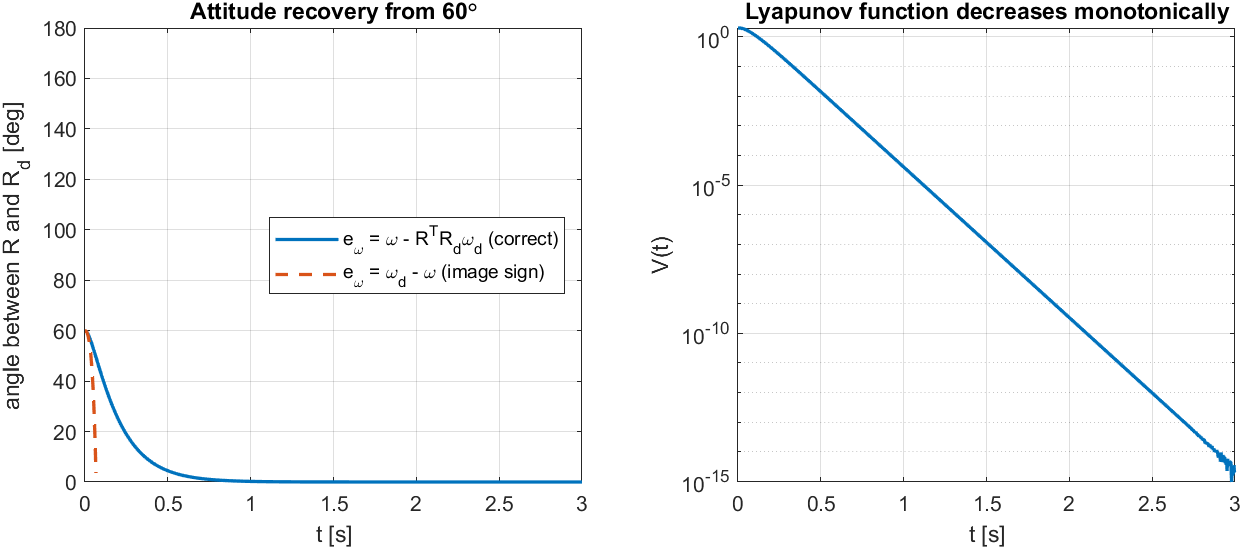
\includegraphics[width=0.92\linewidth]{step7_attitude_recovery.png}
  \caption{Toy model, Model~1 step~7. Left: recovery from 60$^\circ$ with the corrected and the original sign of
  $\ve_\omega$. Right: the Lyapunov function $V$ decreases monotonically with the corrected law.}
  \label{fig:m1-att}
\end{figure}

\begin{projbox}
This is the fast inner loop: ``I should be leaning like $R_d$ but I am leaning like $\hR$, so which way do I
twist?''. It works directly with rotation matrices, so it handles any orientation without gimbal lock. That is the
central claim of our README (``Euler-angle-free''). In code it is \code{compute\_attitude\_error()},
\code{compute\_angular\_velocity\_error()} and \code{compute\_moment()} in \code{so3\_controller.py}. In the current
ROS~2 interface the node publishes $\vF_d$, $\ve_R$ and $\vtau$ as diagnostics and sends velocity commands, and ArduPilot
executes its own inner loop. The equations are the same.
\end{projbox}

\begin{codebox}
\intoy \code{step7\_attitude\_control.m}, \code{lib/attitude\_control.m}.
\end{codebox}

% ---------------------------------------------------------------------
\subsection{Block 8 --- Actuator commands and feedback}
\label{sec:m1b8}
% ---------------------------------------------------------------------

\begin{eqbox}{cPlant}{Equations M1.24 -- M1.25 \quad Control allocation and motor speeds}
\begin{align}
  \begin{bmatrix}T\\ \vtau\end{bmatrix}&=\Gamma\,\vf,\qquad
  \Gamma=\begin{bmatrix}1&1&1&1\\ y_1&y_2&y_3&y_4\\ -x_1&-x_2&-x_3&-x_4\\ \kappa_1c_m&\kappa_2c_m&\kappa_3c_m&\kappa_4c_m\end{bmatrix} \tag{M1.24}\label{eq:m1.24}\\
  \Omega_i&=\sqrt{\frac{\big(\Gamma^{-1}\vu\big)_i}{k_f}}\quad\text{clipped to }[\Omega_{\min},\Omega_{\max}] \tag{M1.25}\label{eq:m1.25}
\end{align}
\end{eqbox}

\begin{dimtable}
\vf=[f_1..f_4] & individual rotor thrusts & \R^4 & N\\
(x_i,y_i) & rotor position in the body frame & \R^2 & m\\
\kappa_i & spin sign ($-1$ CCW, $+1$ CW) & \{\pm1\} & --\\
c_m & yaw torque per newton of thrust & \R & m\\
\Gamma & allocation (mixer) matrix & \R^{4\times4} & --, m\\
k_f & thrust constant & \R & N\,s$^2$\\
\vOm & rotor speeds & \R^4 & rad/s\\
\end{dimtable}

\subsubsection*{Derivation}

Each rotor $i$ produces a force $f_i\ve_3$ at $\bm r_i=[x_i,y_i,0]^\top$. Summing:
\begin{itemize}
  \item total thrust $T=\sum_if_i$;
  \item torque $\sum_i\bm r_i\times f_i\ve_3=\sum_if_i[y_i,\,-x_i,\,0]^\top$, which gives the roll and pitch rows;
  \item yaw: the air resists the spinning propeller, so the motor reacts on the body with $\kappa_ic_mf_i$ about $\ve_3$.
        CCW rotors push the body clockwise.
\end{itemize}
This gives \eqref{eq:m1.24}. Momentum theory gives a rotor thrust proportional to the square of the tip speed,
$f_i=k_f\Omega_i^2$. Inverting both relations gives \eqref{eq:m1.25}. Motors can neither reverse nor exceed their maximum
speed, so $\Omega_i$ is clipped, and the wrench actually produced is $\Gamma k_f\vOm^2$.

For the Iris (ArduPilot Quad-X: 1 front-right CCW, 2 back-left CCW, 3 front-left CW, 4 back-right CW):
\[
\Gamma=\begin{bmatrix}1&1&1&1\\-0.22&0.22&0.22&-0.22\\-0.13&0.13&-0.13&0.13\\-0.016&-0.016&0.016&0.016\end{bmatrix}.
\]

\begin{toybox}[hover and the roll correction of block 7]
\textbf{Hover} $\vu=[14.715,0,0,0]$: $f_i=14.715/4=3.679$\,N,
$\Omega_i=\sqrt{3.679/8.549\times10^{-6}}=656$\,rad/s $=6264$\,rpm.

\textbf{Roll correction} $\vu=[14.491,-0.8546,0,0]$: by symmetry $f_1=f_4=a$ and $f_2=f_3=b$, with
$2a+2b=14.491$ and $0.44(b-a)=-0.8546$. So $a=4.594$\,N and $b=2.652$\,N, i.e.\\
$\vOm=[733,\,557,\,557,\,733]$\,rad/s. The right-side rotors (1, 4) speed up and the drone rolls back to level.
\end{toybox}

\begin{figure}[h]
  \centering
  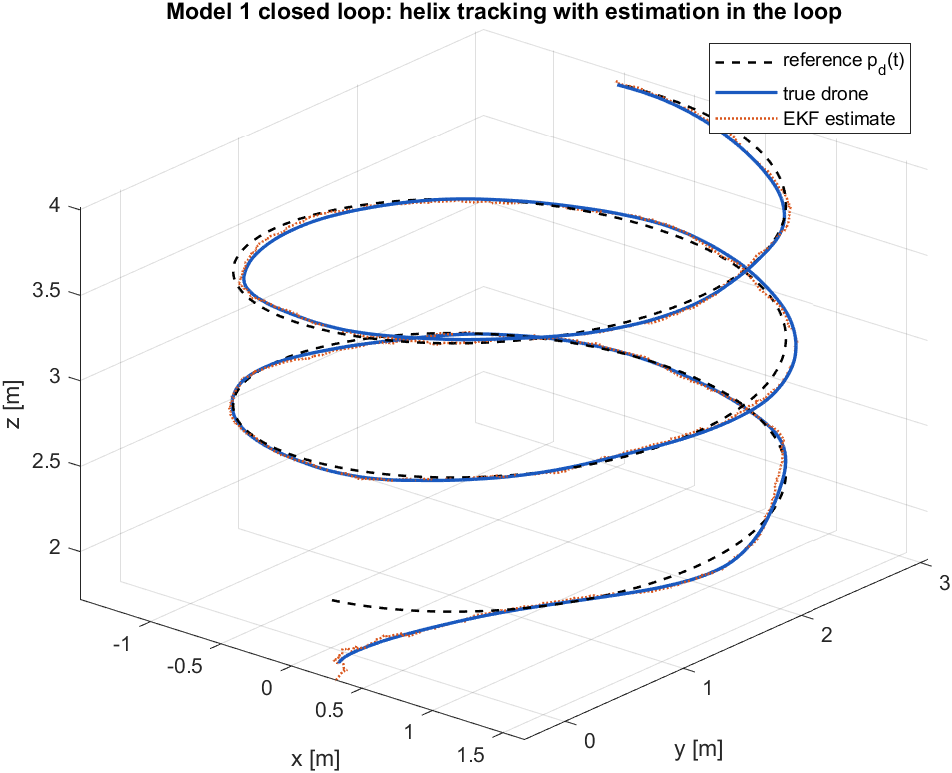
\includegraphics[width=0.43\linewidth]{step8_closed_loop_3d.png}\hfill
  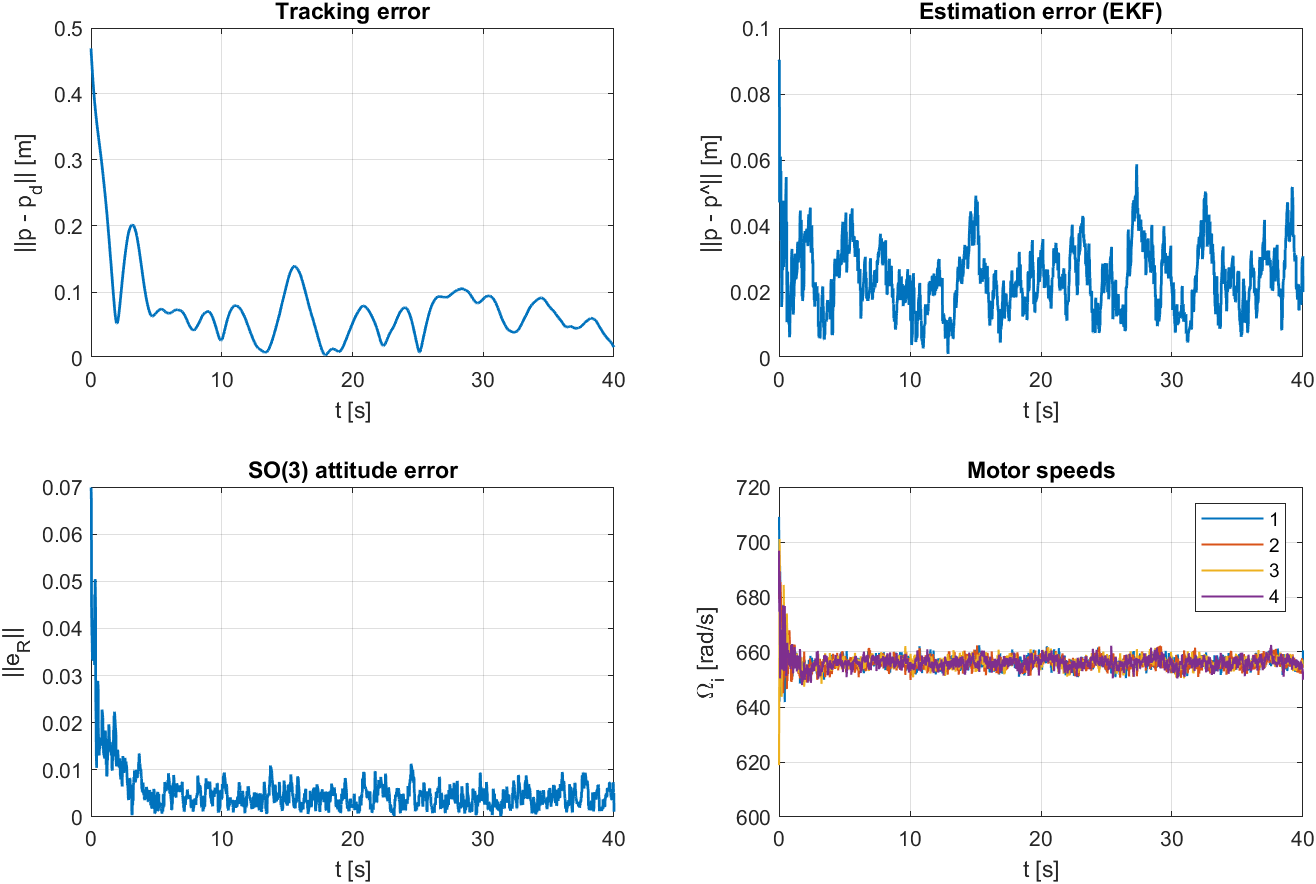
\includegraphics[width=0.55\linewidth]{step8_closed_loop_signals.png}
  \caption{Toy model, Model~1 step~8: the complete loop (truth $\to$ sensors $\to$ EKF $\to$ blocks 5--7 $\to$
  allocation $\to$ truth) tracking a climbing helix in wind. After the transient: tracking RMSE 6.8\,cm,
  estimation RMSE 2.6\,cm, motor speeds 619--709\,rad/s.}
  \label{fig:m1-loop}
\end{figure}

\begin{projbox}
The flight controller does not ``send a torque''. It sends four motor speeds. This block is ArduPilot's motor
mixer. When our node commands velocities (\code{/ap/v1/cmd\_vel}), ArduPilot runs blocks 5--8 internally. When it
commands force and moment, this is the matrix that turns them into ESC signals. The closed loop in
\cref{fig:m1-loop} is the whole of Model~1 working together: the arrow from block~8 back to block~1.
\end{projbox}

\begin{codebox}
\intoy \code{step8\_actuators\_feedback.m}, \code{lib/motor\_allocation.m}.
\end{codebox}

% ---------------------------------------------------------------------
\subsection{Recap of Model 1}
\label{sec:m1recap}
% ---------------------------------------------------------------------

\begin{center}\small
\begin{tabularx}{\linewidth}{@{}c >{\raggedright\arraybackslash}p{2.9cm} >{\raggedright\arraybackslash}p{3.2cm} >{\raggedright\arraybackslash}p{3.0cm} X@{}}
\toprule
\textbf{\#} & \textbf{Block} & \textbf{In} & \textbf{Out} & \textbf{The idea in one sentence}\\
\midrule
1 & Nonlinear dynamics & thrust $T$, torque $\vtau$ & motion $\vp,\vv,R,\vw$ & Newton and Euler: push along the body $z$-axis, gravity pulls down, torque spins the body.\\
2 & Linearization & operating point & $A$, $B$ & Near any flight condition the drone behaves like a linear system.\\
3 & Error dynamics & $A$, $B$, $\Delta t$ & $F$ & Small errors evolve linearly; without feedback they grow.\\
4 & Error-state EKF & $\vu_k$, sensors $\vz_k$ & estimate $\hx_k$, $P_k$ & Predict with physics, correct with camera and IMU, weighting by trust.\\
5 & Position control & $\hp,\hv$, reference & $\va_d$ & Accelerate towards the target like a spring with a damper.\\
6 & Force \& attitude & $\va_d$, yaw & $\vF_d$, $R_d$ & To accelerate sideways, lean; thrust direction $=$ desired force direction.\\
7 & SO(3) attitude & $\hR,\hw,R_d,\vF_d$ & $\vtau$, $T$ & Twist along the gradient of the attitude error; energy always decreases.\\
8 & Allocation & $T$, $\vtau$ & $\Omega_1..\Omega_4$ & Split thrust and torque among four rotors; speed $\propto\sqrt{\text{thrust}}$.\\
\bottomrule
\end{tabularx}
\end{center}

% =====================================================================
\section{Model 2 --- Data-Driven Model and Optimal Control}
\label{sec:model2}
% =====================================================================

Model~1 needs the physics: $m$, $J$, rotor constants. Model~2 asks a different question: \emph{if we only had
recorded flight data, could we still build a good controller?} It learns a discrete-time linear model from
data (blocks 1--2). It then designs an optimal controller on that model in two ways: LQR, which is optimal and
simple but unaware of limits (blocks 3--6), and MPC, which is optimal and respects limits but needs an optimizer
(blocks 7--9). Finally it flies the real, nonlinear drone with the result (block~10).

All matrices here are \emph{discrete-time}: $\vx_{k+1}=A\vx_k+B\vu_k$ with $\Delta t=0.04$\,s, which is the 25\,Hz
\code{control\_rate} of \code{controller.yaml}.

% ---------------------------------------------------------------------
\subsection{Block 1 --- Nonlinear flight data}
\label{sec:m2b1}
% ---------------------------------------------------------------------

\begin{eqbox}{cPlant}{Equation M2.1 \quad Sampled state and input (deviation from hover)}
\begin{equation}
  \vx_k=\begin{bmatrix}\vp(t_k)-\vp_{\mathrm{ref}}\\ \vv(t_k)\\ \Log\big(R(t_k)\big)\\ \vw(t_k)\end{bmatrix}\in\R^{12},\qquad
  \vu_k=\begin{bmatrix}T(t_k)-mg_0\\ \vtau(t_k)\end{bmatrix}\in\R^{4},\qquad t_k=k\,\Delta t . \tag{M2.1}\label{eq:m2.1}
\end{equation}
\end{eqbox}

\begin{dimtable}
\vx_k & state deviation at sample $k$ & \R^{12} & m, m/s, rad, rad/s\\
\vu_k & input deviation at sample $k$ & \R^{4} & N, N\,m\\
\vp_{\mathrm{ref}} & hover point & \R^3 & m ($[0,0,2]$)\\
\Delta t & sample time & \R & s (0.04)\\
N & number of samples in a flight & \mathbb N & -- (625 per 25\,s flight)\\
\end{dimtable}

\subsubsection*{Derivation and reasoning}

\textbf{Operating point.} Hover is an equilibrium of \eqref{eq:m1.1}--\eqref{eq:m1.4}: with $\vv=0$, $R=I$, $\vw=0$,
$T=mg_0$, $\vtau=0$, every derivative is zero. Linearizing about it gives $\delta\dot{\vx}=A_c\delta\vx+B_c\delta\vu$
with \emph{no constant term}. Measuring the state and input as deviations from hover is what lets the pure linear
form $\vx_{k+1}=A\vx_k+B\vu_k$ fit the data. If the raw thrust $T$ were used, gravity would appear as a constant
offset that this form cannot represent (correction~6 in \cref{sec:errata}).

\textbf{Attitude as a vector.} DMDc needs vectors. $\Log(R)$ turns the $3\times3$ rotation into the 3-vector rotation
angle, which near hover is the familiar (roll, pitch, yaw).

\textbf{Sampling.} The computer applies $\vu_k$ and holds it for $\Delta t$ (zero-order hold). Hence the natural model
is discrete.

\textbf{Persistent excitation.} A free quadrotor is unstable (\cref{sec:m1b3}), so data is always recorded with some
stabilising pilot in the loop, here a simple PD controller (the role ArduPilot plays). If the input were
\emph{only} feedback, $\vu_k=-K_0\vx_k$, the rows of $U$ would be linear combinations of the rows of $X$. The data could
not separate ``the drone'' from ``the pilot''. A small random excitation is therefore added on top
($\pm2$\,N thrust, $\pm0.03$\,N\,m torque, held for 0.2\,s), which makes the stacked data matrix full rank.

\begin{toybox}[the recorded data set]
Five flights of 25\,s at 25\,Hz, each starting from a random point near $[0,0,2]$\,m: $5\times625$ samples of
$\vx_k\in\R^{12}$ and $\vu_k\in\R^4$, with small logging noise. Flights 1--4 are used for identification and
flight~5 is kept for validation. The largest roll/pitch in the data is $6.5^\circ$, well inside the
near-linear range of \cref{sec:m1b2}.
\end{toybox}

\begin{figure}[h]
  \centering
  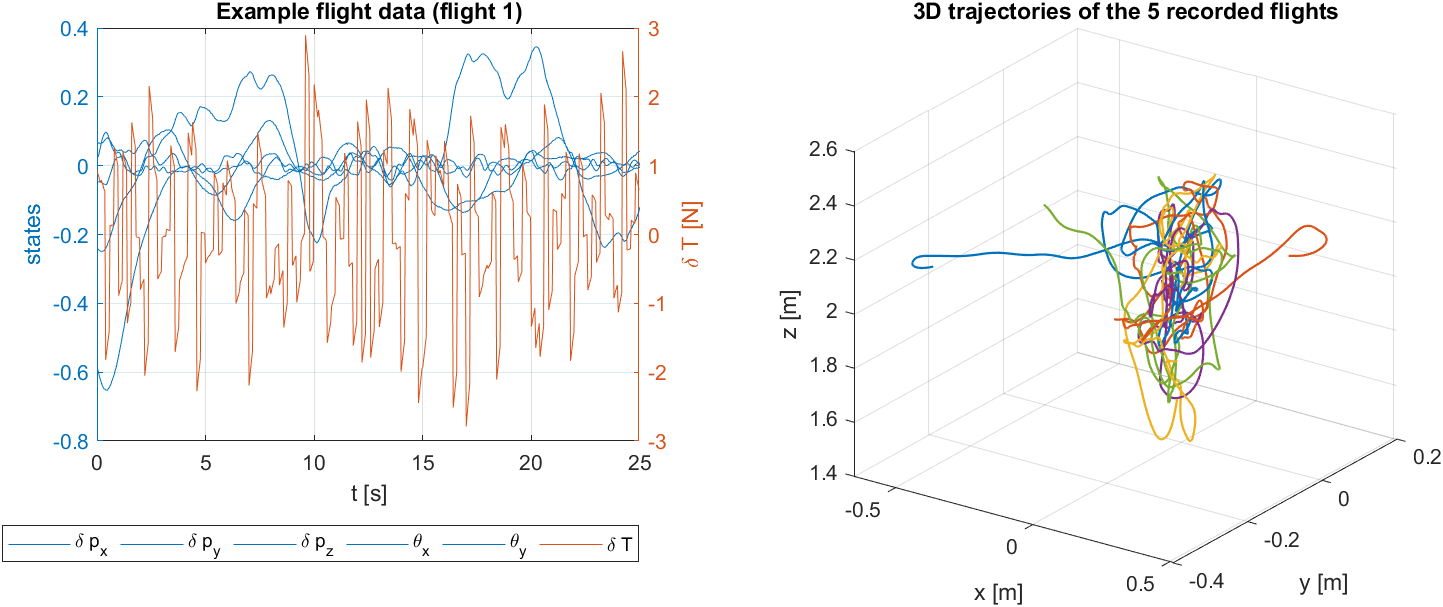
\includegraphics[width=0.92\linewidth]{step1_flight_data.png}
  \caption{Toy model, Model~2 step~1: example time histories and the 3D tracks of the five recorded flights.}
\end{figure}

\begin{projbox}
In the project, this block is a \code{ros2 bag record} of \code{/ap/v1/pose/filtered},
\code{/ap/v1/twist/filtered} and the commands we send, recorded from ArduPilot SITL in Gazebo or from the real
drone. Nothing about mass or inertia needs to be known.
\end{projbox}

\begin{codebox}
\intoy \code{model2\_dmdc\_lqr\_mpc/step1\_flight\_data.m}, \code{lib/state\_to\_dev.m}, \code{lib/baseline\_pilot.m}.
\end{codebox}

% ---------------------------------------------------------------------
\subsection{Block 2 --- DMDc: Dynamic Mode Decomposition with control}
\label{sec:m2b2}
% ---------------------------------------------------------------------

\begin{eqbox}{cOuter}{Equations M2.2 -- M2.4 \quad Snapshot matrices and least-squares model}
\begin{align}
  X=\big[\vx_1\ \cdots\ \vx_{N-1}\big],\quad X^+&=\big[\vx_2\ \cdots\ \vx_{N}\big],\quad U=\big[\vu_1\ \cdots\ \vu_{N-1}\big] \tag{M2.2}\label{eq:m2.2}\\
  \big[\,A\ \ B\,\big]&=X^+\begin{bmatrix}X\\ U\end{bmatrix}^{\dagger} \tag{M2.3}\label{eq:m2.3}\\
  \vx_{k+1}&\approx A\,\vx_k+B\,\vu_k \tag{M2.4}\label{eq:m2.4}
\end{align}
\end{eqbox}

\begin{dimtable}
X,\ X^+ & state snapshots and the same shifted by one sample & \R^{12\times(N-1)} & mixed\\
U & input snapshots & \R^{4\times(N-1)} & N, N\,m\\
\Omega=[X;U] & stacked regressor matrix & \R^{16\times(N-1)} & mixed\\
\Omega^\dagger & pseudo-inverse of $\Omega$ & \R^{(N-1)\times16} & mixed\\
A & learned discrete state matrix & \R^{12\times12} & --\\
B & learned discrete input matrix & \R^{12\times4} & mixed\\
\end{dimtable}

\subsubsection*{Derivation}

We want the pair $G=[A\ B]$ for which $\vx_{k+1}=A\vx_k+B\vu_k=G\,[\vx_k;\vu_k]$ holds as well as possible for
\emph{every} recorded sample. Written for all samples at once, this is $X^+\approx G\,\Omega$. The least-squares choice
minimises the sum of squared one-step prediction errors:
\[
  \min_G\ \big\|X^+-G\,\Omega\big\|_F^2 .
\]
Setting the gradient to zero, $-2\,(X^+-G\Omega)\Omega^\top=0$, gives the \emph{normal equations}
$G\,\Omega\Omega^\top=X^+\Omega^\top$. If $\Omega$ has full row rank (16, guaranteed by the excitation), the
$16\times16$ matrix $\Omega\Omega^\top$ is invertible and
\[
  G=X^+\Omega^\top\big(\Omega\Omega^\top\big)^{-1}=X^+\Omega^\dagger .
\]
In practice $\Omega^\dagger$ is computed from the SVD $\Omega=U_\Omega\Sigma V_\Omega^\top$ as
$V_\Omega\Sigma^{-1}U_\Omega^\top$, and tiny singular values can be truncated to suppress noise
(Proctor, Brunton \& Kutz, 2016). Splitting the columns of $G$ gives $A$ (first 12) and $B$ (last 4).

\textbf{Relation to Model~1.} If the data came from the linearized physics, the exact answer would be the
zero-order-hold discretization of \eqref{eq:AB}:
$A=e^{A_c\Delta t}$, $B=\int_0^{\Delta t}e^{A_cs}ds\,B_c$. DMDc recovers these numbers from data alone.

\begin{toybox}[a scalar system by hand]
True system $x_{k+1}=0.9x_k+0.5u_k$. Three recorded steps:
$X=[1,\ 1.4,\ 0.76]$, $X^+=[1.4,\ 0.76,\ 0.934]$, $U=[1,\ -1,\ 0.5]$.
\[
\Omega\Omega^\top=\begin{bmatrix}3.5376&-0.02\\-0.02&2.25\end{bmatrix},\qquad
X^+\Omega^\top=\begin{bmatrix}3.17384&1.107\end{bmatrix},
\]
\[
[a\ \ b]=\frac{1}{7.9592}\begin{bmatrix}3.17384&1.107\end{bmatrix}\begin{bmatrix}2.25&0.02\\0.02&3.5376\end{bmatrix}
=\begin{bmatrix}0.9000&0.5000\end{bmatrix}.
\]
The true model is recovered exactly, because the data is noise-free.

\textbf{The drone} (2500 snapshots, rank$[X;U]=16$):
\begin{center}\small
\begin{tabular}{@{}llrr@{}}
\toprule
entry & physical meaning & DMDc & physics (ZOH)\\
\midrule
$A_{1,4}$ & $\Delta t$ (position from velocity) & 0.0399 & 0.0400\\
$A_{4,8}$ & $\approx g_0\Delta t$ ($v_x$ from pitch) & 0.3909 & 0.3924\\
$A_{5,7}$ & $\approx-g_0\Delta t$ ($v_y$ from roll) & $-0.3862$ & $-0.3924$\\
$B_{6,1}$ & $\Delta t/m$ ($v_z$ from thrust) & 0.0268 & 0.0267\\
$B_{10,2}$ & $\Delta t/J_x$ (roll rate from roll torque) & 2.0007 & 2.0000\\
$B_{12,4}$ & $\Delta t/J_z$ (yaw rate from yaw torque) & 1.0096 & 1.0000\\
\bottomrule
\end{tabular}
\end{center}
Overall $\|A-A_{\text{phys}}\|/\|A_{\text{phys}}\|=0.95\%$ and $\|B-B_{\text{phys}}\|/\|B_{\text{phys}}\|=0.81\%$. On the unseen
flight, the 1-second-ahead position prediction error is 1.21\,cm, compared with 1.14\,cm for the exact physics
model. The learned mass is $\Delta t/B_{6,1}=1.49$\,kg and the learned roll inertia is $\Delta t/B_{10,2}=0.0200$\,kg\,m$^2$.
\end{toybox}

\begin{figure}[h]
  \centering
  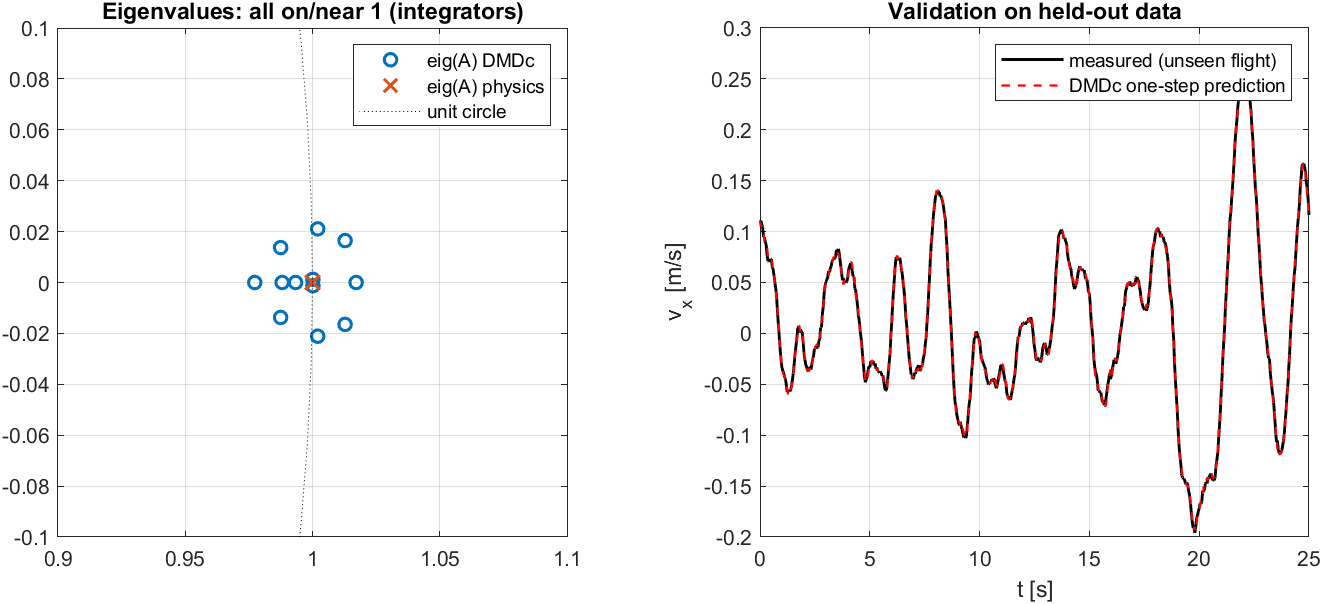
\includegraphics[width=0.9\linewidth]{step2_dmdc_validation.png}
  \caption{Toy model, Model~2 step~2. Left: eigenvalues of the learned and physical $A$, all at or near $1$
  (integrators). Right: one-step predictions on a flight that was \emph{not} used for learning.}
\end{figure}

\begin{projbox}
DMDc is ``curve fitting for dynamics''. It looks at thousands of moments of the form ``the drone was here, we
pushed like this, and 40\,ms later it was there'', and finds the single linear rule that explains them best. For our
drone this means we can re-identify the model whenever something changes (a heavier camera, a new battery, a
different frame) simply by flying for two minutes.
\end{projbox}

\begin{codebox}
\intoy \code{step2\_dmdc.m}, \code{lib/dmdc.m}, \code{lib/c2d\_zoh.m}.
\end{codebox}

% ---------------------------------------------------------------------
\subsection{Block 3 --- Bellman equation (optimal control)}
\label{sec:m2b3}
% ---------------------------------------------------------------------

\begin{eqbox}{cGuid}{Equations M2.5 -- M2.7 \quad Cost, Bellman equation, quadratic value function}
\begin{align}
  J&=\sum_{k=0}^{\infty}\big(\vx_k^\top Q\,\vx_k+\vu_k^\top R\,\vu_k\big) \tag{M2.5}\label{eq:m2.5}\\
  V(\vx_k)&=\min_{\vu_k}\Big[\vx_k^\top Q\vx_k+\vu_k^\top R\vu_k+V(\vx_{k+1})\Big],\qquad \vx_{k+1}=A\vx_k+B\vu_k \tag{M2.6}\label{eq:m2.6}\\
  V(\vx)&=\vx^\top P\,\vx \tag{M2.7}\label{eq:m2.7}
\end{align}
\end{eqbox}

\begin{dimtable}
J & total cost of a flight & \R & -- (dimensionless)\\
Q & state weight, $Q=Q^\top\succeq0$ & \R^{12\times12} & 1/(unit of $x_i$)$^2$\\
R & input weight, $R=R^\top\succ0$ & \R^{4\times4} & 1/N$^2$, 1/(N\,m)$^2$\\
V(\vx) & value function: lowest possible cost from state $\vx$ & \R & --\\
P & value matrix, $P=P^\top\succeq0$ & \R^{12\times12} & as $Q$\\
\end{dimtable}

\subsubsection*{Derivation}

\textbf{(M2.5) The cost.} $\vx^\top Q\vx$ is a weighted sum of squared errors and $\vu^\top R\vu$ a weighted sum of
squared effort. Minimising $J$ trades accuracy against effort. We choose the weights by \emph{Bryson's rule},
$Q_{ii}=1/x_{i,\max}^2$ and $R_{jj}=1/u_{j,\max}^2$, where $x_{i,\max}$ is the largest acceptable deviation. A 50\,cm
position error then costs as much as a 1\,m/s speed error, a $0.2$\,rad tilt, or 5\,N of extra thrust.

\textbf{(M2.6) Principle of optimality} (Bellman). Split the infinite sum into the first step and the rest:
\[
  V(\vx_k)=\min_{\vu_k,\vu_{k+1},\dots}\Big[\ell(\vx_k,\vu_k)+\sum_{j>k}\ell(\vx_j,\vu_j)\Big]
  =\min_{\vu_k}\Big[\ell(\vx_k,\vu_k)+\underbrace{\min_{\vu_{k+1},\dots}\sum_{j>k}\ell(\vx_j,\vu_j)}_{V(\vx_{k+1})}\Big].
\]
Whatever the first move is, the remaining moves must be optimal for the state it leads to. Otherwise we could
improve them and lower the total. The infinite-dimensional problem collapses to a one-step problem.

\textbf{(M2.7) Quadratic value function.} Suppose $V(\vx_{k+1})=\vx_{k+1}^\top P\vx_{k+1}$. The bracket in \eqref{eq:m2.6}
is then a quadratic function of $\vu_k$; its minimiser is linear in $\vx_k$ (block~4), and the minimum value is again a
quadratic form in $\vx_k$ (block~5). The quadratic shape is preserved by the Bellman equation, so the guess
$V=\vx^\top P\vx$ is self-consistent, and all that remains is to find $P$.

\begin{toybox}[one Bellman step by hand]
$x_{k+1}=1.1x_k+0.5u_k$ (unstable: grows 10\% per step), $q=r=1$, next-step value $V(x)=1\cdot x^2$, current $x=1$:
\[
  \text{RHS}(u)=1+u^2+(1.1+0.5u)^2,\qquad \frac{d}{du}=2u+(1.1+0.5u)=0\ \Rightarrow\ u^*=-\frac{1.1}{2.5}=-0.44,
\]
\[
  V(1)=1+0.1936+(1.1-0.22)^2=1.968 .
\]
\code{fminsearch} on the same function returns $u^*=-0.4400$ and $V=1.9680$.

\textbf{Drone} (DMDc model, $V_{\text{next}}=\vx^\top Q\vx$, drone 50/30/20\,cm off target): brute-force minimisation over
$\vu\in\R^4$ and the closed form both give $\vu^*=[-0.0104,-0.0001,0.0001,0.0000]$ and the same value 3.0393.
Doing nothing ($\vu=0$) costs 14\,593 after 10\,s and keeps growing.
\end{toybox}

\begin{projbox}
$Q$ and $R$ are where \emph{we} write down what ``good flying'' means for our mission. For mapping with a camera we
care about smooth, gentle motion (blur-free images), so tilt and rate errors are weighted heavily and speed is
limited to the \code{max\_velocity} of 1\,m/s. The Bellman equation turns that wish list into a mathematical problem with a
unique best answer.
\end{projbox}

\begin{codebox}
\intoy \code{step3\_bellman\_cost.m}, \code{lib/bellman\_backup.m}.
\end{codebox}

% ---------------------------------------------------------------------
\subsection{Block 4 --- Linear Quadratic Regulator (LQR)}
\label{sec:m2b4}
% ---------------------------------------------------------------------

\begin{eqbox}{cGuid}{Equations M2.8 -- M2.9 \quad Optimal gain and control law}
\begin{align}
  K&=\big(R+B^\top PB\big)^{-1}B^\top PA \tag{M2.8}\label{eq:m2.8}\\
  \vu_k&=-K\,\vx_k \tag{M2.9}\label{eq:m2.9}
\end{align}
\end{eqbox}

\begin{dimtable}
K & state-feedback gain & \R^{4\times12} & N/m, N\,s/m, N\,m/rad, \dots\\
R+B^\top PB & curvature of the one-step cost in $\vu$ & \R^{4\times4} & --\\
\end{dimtable}

\subsubsection*{Derivation}

Insert $V(\vx_{k+1})=(A\vx+B\vu)^\top P(A\vx+B\vu)$ into the bracket of \eqref{eq:m2.6} and differentiate with respect to
$\vu$ (using $\partial(\vu^\top M\vu)/\partial\vu=2M\vu$ for symmetric $M$):
\[
  \frac{\partial}{\partial\vu}\Big[\vx^\top Q\vx+\vu^\top R\vu+(A\vx+B\vu)^\top P(A\vx+B\vu)\Big]
  =2R\vu+2B^\top P(A\vx+B\vu)=\bm0 .
\]
Collecting the $\vu$ terms: $(R+B^\top PB)\,\vu=-B^\top PA\,\vx$. Because $R\succ0$ and $P\succeq0$, the matrix
$R+B^\top PB$ is positive definite. It is therefore invertible, and its positive curvature (the Hessian $2(R+B^\top PB)$)
guarantees a minimum. Hence $\vu^*=-(R+B^\top PB)^{-1}B^\top PA\,\vx=-K\vx$.

\begin{toybox}[the scalar system]
With the converged $P=3.1215$ (block~6): $K=\dfrac{ab\,P}{r+b^2P}=\dfrac{1.1\cdot0.5\cdot3.1215}{1+0.25\cdot3.1215}=0.9643$.
Closed loop: $x_{k+1}=(a-bK)x_k=0.6179\,x_k$. Without control the state grows 10\% per step; with LQR it shrinks
38\% per step.

\textbf{Drone gain} (from block~6), two of its 48 numbers:
\[
\delta T=-9.04\,\delta z-6.92\,v_z,\qquad
\tau_x=0.273\,\delta y+0.321\,v_y-1.444\,\theta_x-0.276\,\omega_x .
\]
If the drone is too high, thrust drops. If it is to the left ($\delta y>0$), it rolls right ($+\tau_x$, which makes $\dot v_y<0$),
but less so if it is already rolled or rolling.

With only a one-step look-ahead ($P=$ one Bellman step from $Q$), the gain gives a spectral radius
$\rho(A-BK)=1.0024>1$: \emph{unstable}. The full infinite-horizon $P$ is essential.
\end{toybox}

\begin{projbox}
The LQR controller is just a table: a $4\times12$ matrix $K$. Every 40\,ms it multiplies the 12 measured errors by $K$
and obtains thrust and three torques. It is extremely cheap to run on the drone and, for the cost we chose,
provably the best possible linear controller. Its weakness is that it knows nothing about limits.
\end{projbox}

\begin{codebox}
\intoy \code{step4\_lqr\_gain.m}, \code{lib/lqr\_gain.m}.
\end{codebox}

% ---------------------------------------------------------------------
\subsection{Block 5 --- Riccati recursion}
\label{sec:m2b5}
% ---------------------------------------------------------------------

\begin{eqbox}{cGuid}{Equation M2.10 \quad Discrete Riccati difference equation}
\begin{equation}
  P_{k+1}=A^\top P_kA-A^\top P_kB\big(R+B^\top P_kB\big)^{-1}B^\top P_kA+Q,\qquad P_0=Q\ \text{(or any terminal weight)} \tag{M2.10}\label{eq:m2.10}
\end{equation}
\end{eqbox}

\begin{dimtable}
P_k & value matrix of a problem with $k$ steps to go & \R^{12\times12} & as $Q$\\
k & iteration index (steps-to-go, \emph{not} time) & \mathbb N & --\\
\end{dimtable}

\subsubsection*{Derivation}

Substitute the optimal input $\vu^*=-K\vx$ back into the bracket of \eqref{eq:m2.6}:
\[
  V_{\text{new}}(\vx)=\vx^\top\Big[Q+K^\top RK+(A-BK)^\top P(A-BK)\Big]\vx .
\]
Expand $(A-BK)^\top P(A-BK)=A^\top PA-A^\top PBK-K^\top B^\top PA+K^\top B^\top PBK$ and add $K^\top RK$:
\[
\begin{aligned}
  &K^\top(R+B^\top PB)K=K^\top B^\top PA\quad\text{(by \eqref{eq:m2.8})}\\
  &\Longrightarrow\ V_{\text{new}}=\vx^\top\big[Q+A^\top PA-A^\top PBK\big]\vx
   =\vx^\top\big[Q+A^\top PA-A^\top PB(R+B^\top PB)^{-1}B^\top PA\big]\vx .
\end{aligned}
\]
This is \eqref{eq:m2.10}. Starting from the terminal cost $P_0$, each application gives the value matrix of a
problem that is one step longer. If $(A,B)$ is stabilisable and $Q\succ0$, the sequence converges to the
infinite-horizon matrix $P_\infty$.

\begin{toybox}[scalar recursion, $a=1.1$, $b=0.5$, $q=r=1$, $P_0=1$]
\[
P_{k+1}=1+1.21P_k-\frac{(0.55P_k)^2}{1+0.25P_k}
\]
\begin{center}\small
\begin{tabular}{l*{10}{c}}
\toprule
$k$ & 0 & 1 & 2 & 3 & 4 & 5 & 6 & 7 & 8 & $\infty$\\
$P_k$ & 1 & 1.968 & 2.596 & 2.905 & 3.036 & 3.089 & 3.109 & 3.117 & 3.120 & 3.1215\\
\bottomrule
\end{tabular}
\end{center}
(35 iterations to $10^{-14}$). For the drone, starting from $P_0=Q$, the relative change falls below $10^{-12}$
after 236 iterations, and $P_\infty$ is positive definite ($\lambda_{\min}=3.27$).
\end{toybox}

\begin{figure}[h]
  \centering
  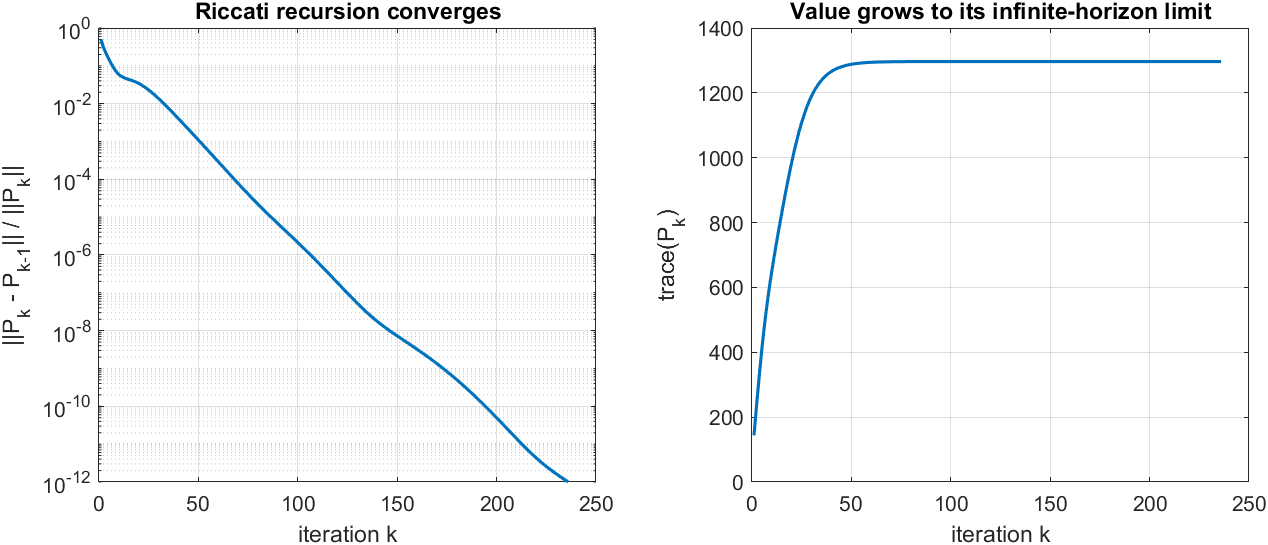
\includegraphics[width=0.85\linewidth]{step5_riccati_convergence.png}
  \caption{Toy model, Model~2 step~5: convergence of the Riccati recursion for the learned drone model.}
\end{figure}

\begin{projbox}
Each iteration lets the controller ``look one step further into the future''. After a few hundred steps, which is 10\,s
of flight at 25\,Hz, looking further no longer changes anything. The drone then plans as if the flight never ends,
which is what an infinite-horizon LQR is.
\end{projbox}

\begin{codebox}
\intoy \code{step5\_riccati\_recursion.m}, \code{lib/riccati\_recursion.m}.
\end{codebox}

% ---------------------------------------------------------------------
\subsection{Block 6 --- DARE: Discrete Algebraic Riccati Equation}
\label{sec:m2b6}
% ---------------------------------------------------------------------

\begin{eqbox}{cGuid}{Equation M2.11 \quad Steady-state Riccati equation}
\begin{equation}
  P=A^\top PA-A^\top PB\big(R+B^\top PB\big)^{-1}B^\top PA+Q \tag{M2.11}\label{eq:m2.11}
\end{equation}
\end{eqbox}

\begin{dimtable}
P & stabilising solution, $P=P^\top\succ0$ & \R^{12\times12} & as $Q$\\
\end{dimtable}

\subsubsection*{Derivation}

If $P_k\to P$, both sides of \eqref{eq:m2.10} tend to the same limit, which gives \eqref{eq:m2.11}. Two further facts make
$P$ useful.

\textbf{Optimal cost.} Using the rearranged form of \eqref{eq:m2.11},
$P=Q+K^\top RK+(A-BK)^\top P(A-BK)$ (from the derivation of block~5), along the closed loop $\vx_{k+1}=(A-BK)\vx_k$:
\[
  \vx_k^\top P\vx_k-\vx_{k+1}^\top P\vx_{k+1}=\vx_k^\top Q\vx_k+\vu_k^\top R\vu_k .
\]
Summing from $k=0$ to $\infty$ (a telescoping sum, and $\vx_k\to0$) gives $J^*=\vx_0^\top P\vx_0$.

\textbf{Direct solution.} Instead of iterating, the optimality conditions $\vu_k=-R^{-1}B^\top\bm\lambda_{k+1}$,
$\bm\lambda_k=Q\vx_k+A^\top\bm\lambda_{k+1}$ (co-state $\bm\lambda_k=P\vx_k$) give the linear pencil
\[
  \begin{bmatrix}I&BR^{-1}B^\top\\0&A^\top\end{bmatrix}\begin{bmatrix}\vx_{k+1}\\ \bm\lambda_{k+1}\end{bmatrix}
  =\begin{bmatrix}A&0\\-Q&I\end{bmatrix}\begin{bmatrix}\vx_k\\ \bm\lambda_k\end{bmatrix}.
\]
Its 12 stable generalised eigenvectors $[X_1;X_2]$ ($|\lambda|<1$) span $\{\bm\lambda=P\vx\}$, so $P=X_2X_1^{-1}$. This is
what \code{lib/dare\_solve.m} implements, so no toolbox is needed.

\begin{toybox}[scalar DARE is a quadratic equation]
$P=1+1.21P-\dfrac{0.3025P^2}{1+0.25P}$. Multiplying by $(1+0.25P)$ and simplifying:
\[
  0.25P^2-0.46P-1=0\ \Longrightarrow\ P=\frac{0.46+\sqrt{0.46^2+1}}{0.5}=3.1215
\]
(the positive root), the limit of the recursion above. The eigenvector solver returns the same value.

\textbf{Drone:} DARE residual $4.2\times10^{-14}$ (relative); agreement with the 236-step recursion $1.1\times10^{-11}$;
closed-loop spectral radius $\rho(A-BK)=0.950<1$, so it is stable. From $\vx_0=[0.5,-0.3,0.2,0,\dots]$: the simulated cost
$\sum(\vx^\top Q\vx+\vu^\top R\vu)=41.4373$ and the predicted $\vx_0^\top P\vx_0=41.4373$ agree.
\end{toybox}

\begin{projbox}
The DARE gives the final $P$ in one shot, and from it the gain $K$ that we would upload to the drone. $P$ is also
reused: it becomes the terminal cost of the MPC (dashed arrow in \cref{fig:flow2}). That is the bridge between the two
branches.
\end{projbox}

\begin{codebox}
\intoy \code{step6\_dare.m}, \code{lib/dare\_solve.m}.
\end{codebox}

% ---------------------------------------------------------------------
\subsection{Block 7 --- Model Predictive Control (MPC)}
\label{sec:m2b7}
% ---------------------------------------------------------------------

\begin{eqbox}{cInner}{Equation M2.12 \quad Finite-horizon constrained optimal control problem}
\begin{equation}
\begin{aligned}
  \min_{\vu_0,\dots,\vu_{N-1}}\ \ &\sum_{k=0}^{N-1}\big(\vx_k^\top Q\vx_k+\vu_k^\top R\vu_k\big)+\vx_N^\top P_f\,\vx_N\\
  \text{subject to}\ \ &\vx_{k+1}=A\vx_k+B\vu_k,\quad \vx_0=\vx(t)\ \text{(measured)},\\
  &\vu_{\min}\le\vu_k\le\vu_{\max},\qquad |C\vx_k|\le\vx_{\max}\quad(k=1..N)
\end{aligned}\tag{M2.12}\label{eq:m2.12}
\end{equation}
\end{eqbox}

\begin{dimtable}
N & prediction horizon & \mathbb N & steps (25 = 1\,s)\\
P_f & terminal weight (here $P_f=P$ from the DARE) & \R^{12\times12} & as $Q$\\
\vu_{\min},\vu_{\max} & input limits (deviation) & \R^4 & N, N\,m\\
C & selects the limited states ($v_x,v_y,v_z$, roll, pitch) & \R^{5\times12} & --\\
\vx_{\max} & state limits & \R^5 & m/s, rad\\
\end{dimtable}

\subsubsection*{Derivation and reasoning}

LQR solves \eqref{eq:m2.5} without limits. Real drones have limits: thrust between roughly 5 and 25\,N, torque that the
rotors can actually produce, the \code{max\_velocity} of 1\,m/s, and a maximum tilt for a camera mount. Adding
constraints destroys the closed-form solution, so MPC solves a \emph{finite} version numerically, from the current
measured state:
\begin{itemize}
  \item the sum stops after $N$ steps, which keeps the problem finite;
  \item the infinite tail $\sum_{k\ge N}$ is replaced by the terminal cost $\vx_N^\top P_f\vx_N$.
\end{itemize}

\textbf{Why $P_f=P$ from the DARE.} By \cref{sec:m2b6}, $\vx_N^\top P\vx_N$ is \emph{exactly} the optimal cost of
the rest of the flight if no constraint is active after step $N$. With this choice, whenever the constraints are not
active, the MPC solution coincides with the LQR solution. Block~8 verifies this numerically.

\begin{toybox}[a two-step problem]
$a=1.1$, $b=0.5$, $q=r=1$, $N=2$, $P_f=3.1215$, $x_0=1$, $|u_k|\le0.5$:
\[
  \min_{u_0,u_1}\ x_0^2+u_0^2+x_1^2+u_1^2+3.1215\,x_2^2\quad\text{s.t.}\ x_{k+1}=1.1x_k+0.5u_k .
\]
\textbf{Drone:} $N=25$ (1\,s look-ahead); $5\le T\le25$\,N, i.e.\ $\delta T\in[-9.715,\,10.285]$\,N; $|\tau_{x,y}|\le0.3$,
$|\tau_z|\le0.05$\,N\,m; $|v_i|\le1$\,m/s; $|\theta_{x,y}|\le0.35$\,rad (20$^\circ$).
\end{toybox}

\begin{projbox}
MPC is a chess player. Every 40\,ms it imagines the next second of flight, finds the best sequence of moves that never
breaks a rule (``never faster than 1\,m/s'', ``never ask a motor for more than it can give''), plays only the first move,
and thinks again. For camera-based mapping, the speed and tilt limits protect image quality.
\end{projbox}

\begin{codebox}
\intoy \code{step7\_mpc\_problem.m}, \code{lib/mpc\_build.m}.
\end{codebox}

% ---------------------------------------------------------------------
\subsection{Block 8 --- Optimization formulation: Quadratic Program}
\label{sec:m2b8}
% ---------------------------------------------------------------------

\begin{eqbox}{cInner}{Equations M2.13 -- M2.15 \quad Stacked prediction, cost and constraints}
\begin{align}
  \mathbf X&=S_x\vx_0+S_u\mathbf U,\qquad
  \mathbf X=\begin{bmatrix}\vx_1\\ \vdots\\ \vx_N\end{bmatrix},\\
  \mathbf U=\begin{bmatrix}\vu_0\\ \vdots\\ \vu_{N-1}\end{bmatrix},\\
  S_x=\begin{bmatrix}A\\ A^2\\ \vdots\\ A^N\end{bmatrix},\\
  S_u=\begin{bmatrix}B&0&\cdots&0\\ AB&B&\cdots&0\\ \vdots&&\ddots&\vdots\\ A^{N-1}B&\cdots&AB&B\end{bmatrix} \tag{M2.13}\label{eq:m2.13}\\[4pt]
  &\min_{\mathbf U}\ \tfrac12\mathbf U^\top H\mathbf U+\bm f^\top\mathbf U,\quad
  H=2\big(S_u^\top\bar QS_u+\bar R\big),\ \ \bm f=2S_u^\top\bar QS_x\vx_0 \tag{M2.14}\label{eq:m2.14}\\[2pt]
  &\text{s.t.}\quad G\mathbf U\le\bm h,\qquad A_{eq}\mathbf U=\bm b_{eq} \tag{M2.15}\label{eq:m2.15}
\end{align}
with $\bar Q=\diag(Q,\dots,Q,P_f)$ and $\bar R=\diag(R,\dots,R)$.
\end{eqbox}

\begin{dimtable}
\mathbf X,\ \mathbf U & stacked predicted states / inputs & \R^{12N},\ \R^{4N} & mixed\\
S_x,\ S_u & prediction matrices & \R^{12N\times12},\ \R^{12N\times4N} & --\\
\bar Q,\ \bar R & block-diagonal weights & \R^{12N\times12N},\ \R^{4N\times4N} & --\\
H,\ \bm f & QP Hessian and linear term & \R^{4N\times4N},\ \R^{4N} & --\\
G,\ \bm h & inequality constraints & \R^{n_c\times4N},\ \R^{n_c} & mixed\\
A_{eq},\ \bm b_{eq} & equality constraints (optional) & \R^{n_e\times4N},\ \R^{n_e} & mixed\\
\end{dimtable}

\subsubsection*{Derivation}

\textbf{(M2.13) Prediction.} Apply $\vx_{k+1}=A\vx_k+B\vu_k$ repeatedly:
$\vx_1=A\vx_0+B\vu_0$, $\vx_2=A^2\vx_0+AB\vu_0+B\vu_1$, and in general
\[
  \vx_k=A^k\vx_0+\sum_{j=0}^{k-1}A^{k-1-j}B\vu_j .
\]
Stacking $k=1..N$ gives \eqref{eq:m2.13}. The future states are \emph{linear} in the unknown inputs.

\textbf{(M2.14) Cost.} The cost of \eqref{eq:m2.12} is $\vx_0^\top Q\vx_0+\mathbf X^\top\bar Q\mathbf X+\mathbf U^\top\bar R\mathbf U$.
Substitute $\mathbf X$:
\[
  \mathbf U^\top\big(S_u^\top\bar QS_u+\bar R\big)\mathbf U+2\,\vx_0^\top S_x^\top\bar QS_u\,\mathbf U+\underbrace{\vx_0^\top(Q+S_x^\top\bar QS_x)\vx_0}_{\text{does not depend on }\mathbf U}.
\]
Dropping the constant and writing it as $\tfrac12\mathbf U^\top H\mathbf U+\bm f^\top\mathbf U$ gives $H$ and $\bm f$ in
\eqref{eq:m2.14}. $H\succ0$ because $\bar R\succ0$, so the problem is \emph{convex}, with a single global minimum
and no local traps.

\textbf{(M2.15) Constraints.} Input limits: $[I;-I]\,\mathbf U\le[\mathbf U_{\max};-\mathbf U_{\min}]$. State limits
$|\bar C\mathbf X|\le\bar{\vx}_{\max}$ become
$\bar CS_u\mathbf U\le\bar{\vx}_{\max}-\bar CS_x\vx_0$ and $-\bar CS_u\mathbf U\le\bar{\vx}_{\max}+\bar CS_x\vx_0$.
Stacking everything gives $G\mathbf U\le\bm h(\vx_0)$. Equality constraints appear, for example, as a terminal
condition $\vx_N=0$, i.e.\ (last block row of $S_u$)$\,\mathbf U=-A^N\vx_0$, or in the ``sparse'' formulation, where both
$\mathbf X$ and $\mathbf U$ are unknowns and the dynamics themselves are the equalities.

\textbf{Solver.} The toy model solves the QP with a primal--dual interior-point method (\code{lib/qp\_solve.m}).
It applies Newton steps on the KKT conditions $H\mathbf U+\bm f+G^\top\bm z+A_{eq}^\top\bm y=0$, $G\mathbf U+\bm s=\bm h$,
$s_iz_i=0$, keeping $\bm s,\bm z>0$. It replaces \code{quadprog}, so no Optimization Toolbox is needed.

\begin{toybox}[the two-step problem of block 7, solved by hand]
\[
S_x=\begin{bmatrix}1.1\\1.21\end{bmatrix},\quad S_u=\begin{bmatrix}0.5&0\\0.55&0.5\end{bmatrix},\quad
\bar Q=\diag(1,\,3.1215),
\]
\[
H=2\left(\begin{bmatrix}1.1942&0.8584\\0.8584&0.7804\end{bmatrix}+I\right)=\begin{bmatrix}4.3885&1.7168\\1.7168&3.5607\end{bmatrix},\qquad
\bm f=\begin{bmatrix}5.2547\\3.7770\end{bmatrix}.
\]
\begin{itemize}
\item \textbf{No limits:} $\mathbf U^*=-H^{-1}\bm f=[-0.9643,\ -0.5958]$. The first move equals the LQR move
      $-Kx_0=-0.9643$ \emph{exactly}, as promised by $P_f=P$.
\item \textbf{With $|u|\le0.5$:} $\mathbf U^*=[-0.5,\ -0.5]$. Both limits are active and the KKT multipliers are positive.
\item \textbf{With $A_{eq}\mathbf U=b_{eq}$ forcing $x_2=0$} ($[0.55\ \ 0.5]\,\mathbf U=-1.21$): $\mathbf U^*=[-1.3057,\ -0.9837]$.
      Check: $0.55(-1.3057)+0.5(-0.9837)=-1.21$.
\end{itemize}
\textbf{Drone ($N=25$):} 100 decision variables and 450 inequality constraints. For a 5\,cm offset (no limit active) the
MPC input equals $-K\vx_0$ to all printed digits. For a 2\,m offset the unconstrained LQR would demand 1.39 times the
allowed input; the QP saturates the thrust at $+10.285$\,N and plans a velocity that touches but never exceeds
1\,m/s. Solved in 10 interior-point iterations (about 8\,ms).
\end{toybox}

\begin{projbox}
Here the physics disappears into a few matrices. To the solver, ``fly the drone well without breaking the
rules'' is just ``find the lowest point of a bowl ($H$, $\bm f$) inside a fence ($G$, $\bm h$)''. Because the bowl has
one bottom, the answer is unique and can be found reliably in milliseconds. That is what makes MPC feasible at 25\,Hz.
\end{projbox}

\begin{codebox}
\intoy \code{step8\_qp\_formulation.m}, \code{lib/mpc\_build.m}, \code{lib/qp\_solve.m}.
\end{codebox}

% ---------------------------------------------------------------------
\subsection{Block 9 --- MPC control input (receding horizon)}
\label{sec:m2b9}
% ---------------------------------------------------------------------

\begin{eqbox}{cInner}{Equation M2.16 \quad Receding-horizon control law}
\begin{equation}
  \mathbf U^*(\vx_k)=\big[\vu_0^*,\ \vu_1^*,\ \dots,\ \vu_{N-1}^*\big]=\arg\min\text{QP}(\vx_k)
  \quad\Longrightarrow\quad \vu_k=\vu_0^*(\vx_k),\quad k\leftarrow k+1 \tag{M2.16}\label{eq:m2.16}
\end{equation}
\end{eqbox}

\begin{dimtable}
\mathbf U^*(\vx_k) & optimal plan computed at time $k$ & \R^{4N} & N, N\,m\\
\vu_0^* & first element of the plan, the only one applied & \R^{4} & N, N\,m\\
\end{dimtable}

\subsubsection*{Derivation and reasoning}

The plan $\mathbf U^*$ is optimal \emph{for the model}. The model is never perfect (it was learned, and wind is not in
it). Re-solving at every sample from the newly measured state $\vx_{k+1}$ turns the open-loop plan into a feedback law
$\vu_k=\kappa(\vx_k)$: errors are corrected 25 times per second instead of accumulating. Applying $\vu_0^*$ and shifting the
horizon forward by one step is the \emph{receding horizon} principle.

\begin{toybox}[8 s on the learned model]
Start 1.5\,m, 1.0\,m and 1.2\,m away from the setpoint. At $k=0$ the plan begins with
$\vu_0^*=[10.285,\,-0.279,\,-0.300,\,0.002]$: full upward thrust and the maximum allowed torque.
Over the run, MPC respects $|v_i|\le1$\,m/s (maximum 1.000), while LQR clipped to the same input limits reaches 1.172\,m/s.
MPC converges to $\|\vx\|=1.3\times10^{-5}$. The state limits never had to be relaxed. The mean solve time is 2.2\,ms
against a 40\,ms budget.
\end{toybox}

\begin{figure}[h]
  \centering
  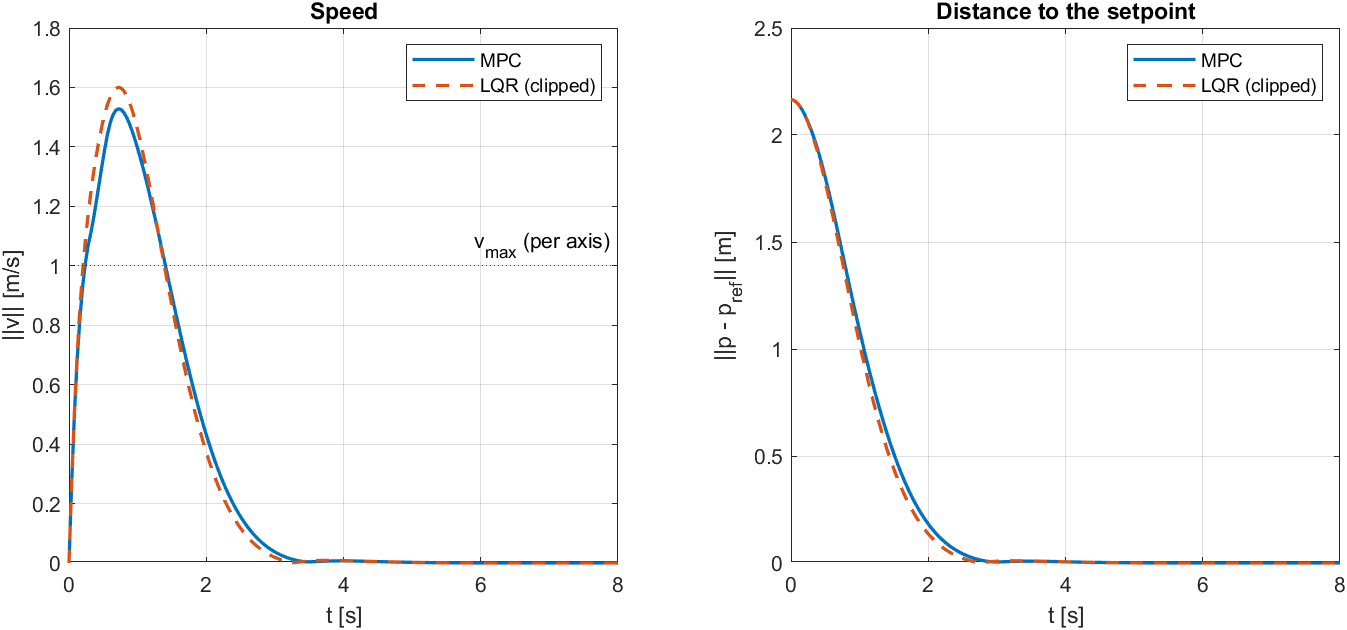
\includegraphics[width=0.9\linewidth]{step9_receding_horizon.png}
  \caption{Toy model, Model~2 step~9: receding-horizon MPC versus input-clipped LQR on the learned model.}
\end{figure}

\begin{projbox}
``Plan one second ahead, act for 40 milliseconds, look again.'' Because the plan is recomputed from fresh EKF
estimates, the MPC inherits the robustness of feedback while still respecting every limit.
\end{projbox}

\begin{codebox}
\intoy \code{step9\_mpc\_control\_input.m}, \code{lib/mpc\_solve.m}.
\end{codebox}

% ---------------------------------------------------------------------
\subsection{Block 10 --- Apply to the drone}
\label{sec:m2b10}
% ---------------------------------------------------------------------

\begin{eqbox}{cPlant}{Equations M2.17 -- M2.18 \quad From optimal input to motor speeds}
\begin{align}
  \vu_k^{\text{abs}}&=\vu_{\text{trim}}+\begin{cases}\vu_0^*(\vx_k)&\text{(MPC)}\\ -K\vx_k&\text{(LQR)}\end{cases}
   =\begin{bmatrix}T_k\\ \vtau_k\end{bmatrix},\qquad \vu_{\text{trim}}=\begin{bmatrix}mg_0\\ \bm0\end{bmatrix} \tag{M2.17}\label{eq:m2.17}\\
  \vf&=\Gamma^{-1}\vu_k^{\text{abs}},\qquad \Omega_i=\sqrt{f_i/k_f}\quad(\text{as in M1.24--M1.25}) \tag{M2.18}\label{eq:m2.18}
\end{align}
\end{eqbox}

\begin{dimtable}
\vu_{\text{trim}} & hover input (operating point) & \R^4 & N, N\,m\\
\vu_k^{\text{abs}} & absolute thrust and torque & \R^4 & N, N\,m\\
\vOm & motor speeds & \R^4 & rad/s\\
\end{dimtable}

\subsubsection*{Derivation}

Models and controllers of Model~2 work in deviations \eqref{eq:m2.1}. The real motors need absolute values, so the
hover trim is added back. The rest is the same allocation as Model~1 (\cref{sec:m1b8}). The loop is closed by
measuring the new state of the \emph{nonlinear} drone (in the project: the EKF of Model~1) and starting block~9 again.
Logged data can also be fed back to block~1 to re-identify the model (outer dashed loop of \cref{fig:flow2}).

\begin{toybox}[one control sample, then a whole flight]
Drone at $[1.5,\,-1.0,\,0.8]$\,m, at rest; target $[0,0,2]$. The MPC gives $\delta\vu=[10.285,\,-0.279,\,-0.300,\,0.002]$, so
$\vu=[25.000,\,-0.279,\,-0.300,\,0.002]$, $\vf=[7.115,\,5.327,\,6.539,\,6.019]$\,N and
$\vOm=[912,\,789,\,875,\,839]$\,rad/s.

\textbf{Nonlinear flight}, 10\,s with gusts and sensor noise, controllers designed only on the DMDc model:
\begin{center}\small
\begin{tabular}{lrrr}
\toprule
controller & max $|v_i|$ [m/s] & error at 10\,s [m] & motor speeds [rad/s]\\
\midrule
MPC & 0.994 & 0.015 & 584 -- 913\\
LQR (clipped) & 1.118 & 0.031 & 613 -- 911\\
\bottomrule
\end{tabular}
\end{center}
Both stabilise the real drone. Only MPC honours \code{max\_velocity} = 1\,m/s.
\end{toybox}

\begin{figure}[h]
  \centering
  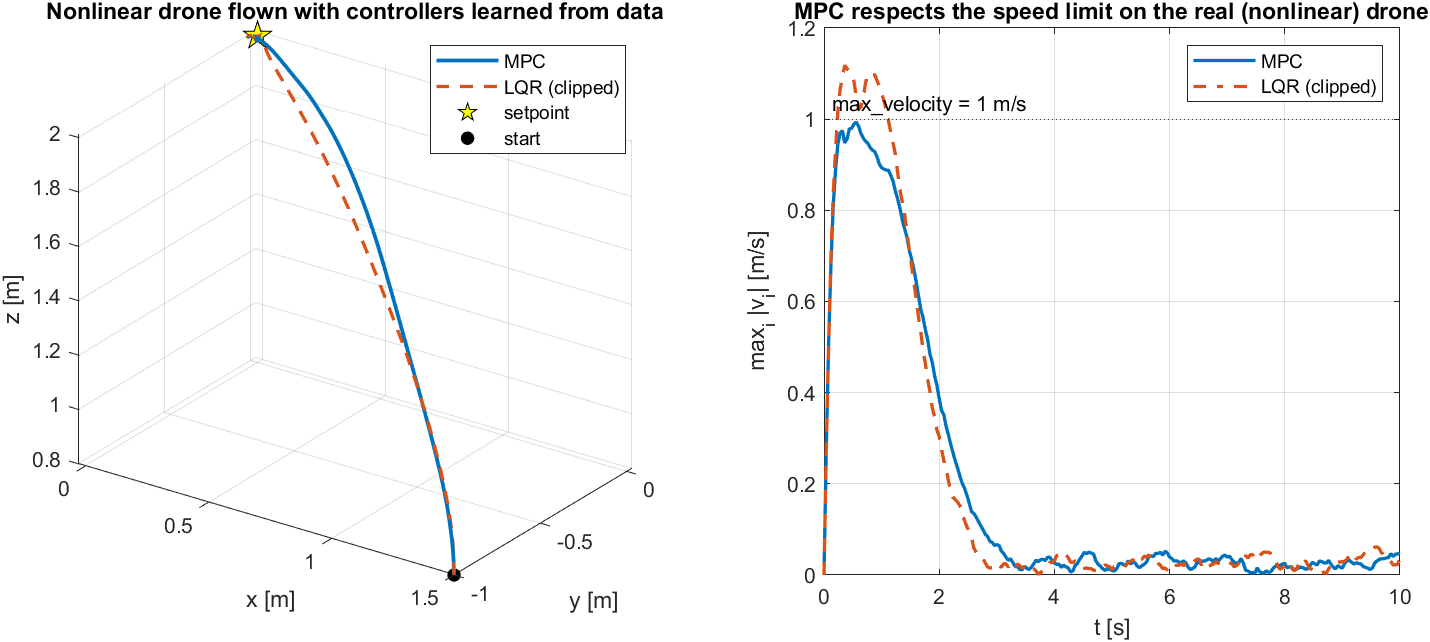
\includegraphics[width=0.95\linewidth]{step10_nonlinear_flight.png}
  \caption{Toy model, Model~2 step~10: the nonlinear drone flown by controllers that were designed on a model learned
  from data.}
\end{figure}

\begin{projbox}
This is the moment of truth: a controller designed on a learned, linear, approximate model flies the real, nonlinear,
gusty, motor-limited drone. In the project this block is the same motor mixer as Model~1, fed through ArduPilot.
\end{projbox}

\begin{codebox}
\intoy \code{step10\_apply\_to\_drone.m}, \code{lib/motor\_allocation.m}.
\end{codebox}

% ---------------------------------------------------------------------
\subsection{Recap of Model 2}
\label{sec:m2recap}
% ---------------------------------------------------------------------

\begin{center}\small
\begin{tabularx}{\linewidth}{@{}c >{\raggedright\arraybackslash}p{2.9cm} >{\raggedright\arraybackslash}p{3.2cm} >{\raggedright\arraybackslash}p{3.0cm} X@{}}
\toprule
\textbf{\#} & \textbf{Block} & \textbf{In} & \textbf{Out} & \textbf{The idea in one sentence}\\
\midrule
1 & Flight data & drone, excitation & $\{\vx_k\},\{\vu_k\}$ & Record what the drone did and what we told it, as deviations from hover.\\
2 & DMDc & $X$, $X^+$, $U$ & $A$, $B$ & Least squares finds the linear rule that best predicts the next sample.\\
3 & Bellman & $A,B,Q,R$ & $V(\vx)=\vx^\top P\vx$ & The best plan from here is the best first move plus the best plan from where it leads.\\
4 & LQR & $A,B,R,P$ & $K$ & Minimising a quadratic gives a linear law $\vu=-K\vx$.\\
5 & Riccati recursion & $P_0$ & $P_\infty$ & Look one more step ahead each iteration until nothing changes.\\
6 & DARE & $A,B,Q,R$ & $P$, final $K$ & Jump straight to that steady state; $\vx_0^\top P\vx_0$ is the optimal cost.\\
7 & MPC & model, limits, $P_f$ & optimisation problem & Plan the next second optimally without breaking any rule.\\
8 & QP & problem, $\vx_0$ & $H,\bm f,G,\bm h$, $\mathbf U^*$ & Substitute the predictions: a convex bowl inside a fence.\\
9 & MPC input & $\vx_k$ & $\vu_0^*$ & Apply only the first move, then re-plan with fresh data.\\
10 & Apply to drone & $\vu_0^*$ or $-K\vx_k$ & $\Omega_1..\Omega_4$ & Add hover thrust back, split among rotors, fly the real drone.\\
\bottomrule
\end{tabularx}
\end{center}

% =====================================================================
\section[How the Two Models Fit Together]{How the Two Models Fit Together in Our Project}
\label{sec:project}
% =====================================================================

\subsection{One drone, two ways of thinking}

\begin{center}\small
\begin{tabularx}{\linewidth}{@{}l X X@{}}
\toprule
 & \textbf{Model 1 (model-based)} & \textbf{Model 2 (data-driven)}\\
\midrule
Where the model comes from & Newton/Euler physics, needs $m$, $J$, rotor constants & Logged flight data (DMDc), no parameters needed\\
Model type & Nonlinear, continuous time, attitude on $\SO$ & Linear, discrete time, around hover\\
Estimation & Error-state EKF fusing camera (VIO) and IMU & Uses the estimate of Model~1 as its measured state\\
Controller & Geometric $\SO$ cascade (position $\to$ attitude) & LQR (gain table) or MPC (online QP)\\
Valid range & Any attitude except upside-down & Near hover (small tilts)\\
Limits / constraints & Only by saturation & Explicit in MPC (\code{max\_velocity}, tilt, thrust)\\
On-board cost per step & A few $3\times3$ products & LQR: one $4\times12$ product; MPC: a QP (about 2\,ms)\\
Code in the repository & \code{so3\_controller.py}, \code{state\_adapter.py} & toy model \code{model2\_dmdc\_lqr\_mpc/}\\
\bottomrule
\end{tabularx}
\end{center}

\subsection{The complete picture}

\begin{enumerate}[leftmargin=*]
  \item The monocular camera produces images, visual odometry turns them into a pose, and the IMU produces rates.
  \item The \textbf{error-state EKF} (M1.10--M1.14) fuses them with the physics (M1.1--M1.4, linearized by M1.5--M1.9)
        into one state estimate $\hx$. This is the ``VIO'' of our title. The same state, with the camera poses, is what
        the 3D map is built from.
  \item Either the \textbf{geometric controller} (M1.15--M1.23) or a \textbf{data-driven LQR/MPC} (M2.5--M2.16) turns
        $\hx$ and the mission waypoints into thrust and torques.
  \item The \textbf{allocation} (M1.24--M1.25 = M2.17--M2.18) turns them into four motor speeds, and the drone moves.
  \item Logged flights can be fed back into DMDc to keep Model~2's $A,B$ up to date.
\end{enumerate}

\subsection{The toy model: \texttt{toy\_model2}}

Every block of both flows is a MATLAB script that prints its \textbf{inputs} and \textbf{outputs} (name, size, unit,
meaning, value). It first reproduces the hand-worked toy example of this document (Part~A) and then passes real data
to the next step (Part~B). Results are saved to \code{results/*.mat} and figures to \code{figures/}. No toolbox is
required: a QP solver and a DARE solver are included.

\begin{center}\small
\begin{tabularx}{\linewidth}{@{}l l X@{}}
\toprule
\textbf{Folder / script} & \textbf{Equations} & \textbf{Inputs $\rightarrow$ outputs}\\
\midrule
\multicolumn{3}{@{}l}{\code{toy\_model2/model1\_nonlinear\_ekf\_so3/} \quad(run \code{run\_all\_model1})}\\
\code{step1\_nonlinear\_dynamics} & M1.1--4 & $\vx,\vu\rightarrow\dot{\vx}$; open-loop flight\\
\code{step2\_taylor\_jacobian} & M1.5--6 & $(\hx,\hu)\rightarrow A,B$; numerical check\\
\code{step3\_local\_error\_dynamics} & M1.7--9 & $A,B,\Delta t\rightarrow F$; linear vs.\ true error\\
\code{step4\_error\_state\_ekf} & M1.10--14 & $\vu_k,\vz_k\rightarrow\hx_k,P_k$\\
\code{step5\_position\_control} & M1.15--16 & $\hp,\hv,\vp_d,\vv_d,\ddot{\vp}_d\rightarrow\ve_p,\ve_v,\va_d$\\
\code{step6\_force\_attitude} & M1.17--19 & $\va_d,\psi_d\rightarrow\vF_d,\vb_{3d},R_d$\\
\code{step7\_attitude\_control} & M1.20--23 & $\hR,\hw,R_d,\vF_d\rightarrow\ve_R,\ve_\omega,\vtau,T$\\
\code{step8\_actuators\_feedback} & M1.24--25 & $T,\vtau\rightarrow\vOm$; full closed loop\\
\midrule
\multicolumn{3}{@{}l}{\code{toy\_model2/model2\_dmdc\_lqr\_mpc/} \quad(run \code{run\_all\_model2})}\\
\code{step1\_flight\_data} & M2.1 & drone + excitation $\rightarrow\{\vx_k\},\{\vu_k\}$\\
\code{step2\_dmdc} & M2.2--4 & $X,X^+,U\rightarrow A,B$\\
\code{step3\_bellman\_cost} & M2.5--7 & $A,B\rightarrow Q,R$; Bellman check\\
\code{step4\_lqr\_gain} & M2.8--9 & $A,B,R,P\rightarrow K$\\
\code{step5\_riccati\_recursion} & M2.10 & $P_0\rightarrow P_\infty$\\
\code{step6\_dare} & M2.11 & $A,B,Q,R\rightarrow P,K$\\
\code{step7\_mpc\_problem} & M2.12 & limits, $N$, $P_f\rightarrow$ MPC problem\\
\code{step8\_qp\_formulation} & M2.13--15 & problem, $\vx_0\rightarrow H,\bm f,G,\bm h,\mathbf U^*$\\
\code{step9\_mpc\_control\_input} & M2.16 & $\vx_k\rightarrow\vu_0^*$ (receding horizon)\\
\code{step10\_apply\_to\_drone} & M2.17--18 & $\vu_0^*$ or $-K\vx_k\rightarrow\vOm$; nonlinear flight\\
\bottomrule
\end{tabularx}
\end{center}

\appendix
% =====================================================================
\section{Proofs of the SO(3) identities}
\label{app:so3}
% =====================================================================

\textbf{\eqref{eq:id1}.} $\skw{\bm a}^\top=-\skw{\bm a}$ by inspection of \eqref{eq:hat}. $\skw{\bm a}\bm a=\bm a\times\bm a=0$, and
$\skw{\bm a}\bm b=\bm a\times\bm b=-\bm b\times\bm a=-\skw{\bm b}\bm a$.

\textbf{\eqref{eq:id2}.} For any $\bm b$: $R\skw{\bm a}R^\top\bm b=R\big(\bm a\times R^\top\bm b\big)=(R\bm a)\times(RR^\top\bm b)=(R\bm a)\times\bm b$,
because a rotation preserves cross products ($R(\bm x\times\bm y)=R\bm x\times R\bm y$ for $\det R=+1$).

\textbf{\eqref{eq:id3}.} Split $M=M_s+M_a$ into symmetric and skew parts. The trace of (symmetric $\times$ skew) is zero, so
$\tr(M\skw{\bm\eta})=\tr(M_a\skw{\bm\eta})$. With $M_a=\skw{\bm m}$, $\bm m=\tfrac12(M-M^\top)^\vee$, a direct calculation gives
$\tr(\skw{\bm m}\skw{\bm\eta})=-2\,\bm m^\top\bm\eta$. Hence $\tr(M\skw{\bm\eta})=-\bm\eta^\top(M-M^\top)^\vee$.

\textbf{Trace and angle.} For $R=\Exp(\theta\bm n)$, \eqref{eq:exp} gives $\tr R=3-(1-\cos\theta)\cdot2=1+2\cos\theta$ (since
$\tr\skw{\bm n}=0$ and $\tr\skw{\bm n}^2=-2$). This is used for $\Psi=1-\cos\varphi$ and for $\Log$.

% =====================================================================
\section{Matrix-calculus rules used}
\label{app:calc}
% =====================================================================

For vectors $\vx,\bm b$ and matrices $M$ (symmetric where stated), $K$, $N$:
\[
\frac{\partial(\bm b^\top\vx)}{\partial\vx}=\bm b,\qquad
\frac{\partial(\vx^\top M\vx)}{\partial\vx}=2M\vx\ (M=M^\top),
\]
\[
\frac{\partial\,\tr(KN)}{\partial K}=N^\top,\qquad
\frac{\partial\,\tr(KMK^\top)}{\partial K}=2KM\ (M=M^\top).
\]
The first two give the LQR gain (Model~2, block~4) and the QP gradient $H\mathbf U+\bm f$ (Model~2, block~8). The last two give the
Kalman gain (Model~1, block~4).

\textbf{Least squares.} $\min_G\|Y-G\Omega\|_F^2$ has gradient $-2(Y-G\Omega)\Omega^\top$. It is zero at
$G=Y\Omega^\top(\Omega\Omega^\top)^{-1}=Y\Omega^\dagger$ when $\Omega$ has full row rank (DMDc, Model~2 block~2).

% =====================================================================
\section{References}
% =====================================================================

\begin{enumerate}[label={[\arabic*]}, leftmargin=*]
\item T.~Lee, M.~Leok, N.\,H.~McClamroch, ``Geometric tracking control of a quadrotor UAV on SE(3)'',
      \emph{IEEE CDC}, 2010 (arXiv:1003.2005). Basis of Model 1, blocks 5--7.
\item J.~Sol\`a, ``Quaternion kinematics for the error-state Kalman filter'', arXiv:1711.02508, 2017. Basis of Model 1, block 4.
\item J.\,L.~Proctor, S.\,L.~Brunton, J.\,N.~Kutz, ``Dynamic mode decomposition with control'',
      \emph{SIAM J.\ Applied Dynamical Systems} 15(1), 2016. Model 2, block 2.
\item D.\,P.~Bertsekas, \emph{Dynamic Programming and Optimal Control}, Vol.~I, Athena Scientific. Model 2, blocks 3--6.
\item J.\,B.~Rawlings, D.\,Q.~Mayne, M.\,M.~Diehl, \emph{Model Predictive Control: Theory, Computation, and Design}, 2nd ed., 2017.
      Model 2, blocks 7--9.
\item T.~Qin, P.~Li, S.~Shen, ``VINS-Mono: a robust and versatile monocular visual-inertial state estimator'',
      \emph{IEEE T-RO}, 2018.
\item ArduPilot SITL and Gazebo Iris model documentation; project parameters from
      \code{controller.yaml} (package \code{drones\_controller}, folder \code{config}).
\end{enumerate}

% =====================================================================
\section{Glossary}
\label{app:glossary}
% =====================================================================

\begin{center}\small
\begin{tabularx}{\linewidth}{@{}l X@{}}
\toprule
\textbf{Term} & \textbf{Meaning}\\
\midrule
ArduPilot SITL & ArduPilot flight software running on a PC (Software-In-The-Loop), flying a simulated drone\\
Attitude & orientation of the drone; here the rotation matrix $R$\\
Body frame & axes fixed to the drone: $x$ forward, $y$ left, $z$ up (FLU)\\
Covariance & matrix of variances/co-variations of errors; the EKF's ``how unsure am I''\\
DARE & Discrete Algebraic Riccati Equation; gives the infinite-horizon LQR solution\\
DMDc & Dynamic Mode Decomposition with control; fits $\vx_{k+1}=A\vx_k+B\vu_k$ to data by least squares\\
EKF & Extended Kalman Filter: Kalman filter applied to a nonlinear model through linearization\\
ENU & East--North--Up world frame used by ArduPilot's ROS 2 topics\\
Error-state & the filter tracks the small error $\delta\vx$, not the full state, so attitude is handled correctly\\
Gazebo & 3D physics simulator in which the Iris quadrotor flies\\
Gimbal lock & singularity of Euler angles at $\pm90^\circ$ pitch; avoided by working with $R$ directly\\
IMU & Inertial Measurement Unit: gyroscope (rates) and accelerometer\\
Innovation & measurement minus what the filter expected to measure\\
Jacobian & matrix of partial derivatives; the ``slope'' of a vector function\\
Kalman gain $K$ & how strongly the estimate is pulled towards a measurement\\
LQR & Linear Quadratic Regulator: optimal linear feedback $\vu=-K\vx$\\
Lyapunov function & energy-like quantity that never increases; proves stability\\
MPC & Model Predictive Control: repeatedly solve a finite-horizon optimal problem with constraints\\
QP & Quadratic Program: minimise a quadratic cost subject to linear constraints\\
Receding horizon & apply only the first planned input, then re-plan one step later\\
RK4 & 4th-order Runge--Kutta: accurate way to step a differential equation forward\\
ROS 2 & Robot Operating System; our controller node talks to ArduPilot through it\\
SO(3) & the set of all 3D rotation matrices ($R^\top R=I$, $\det R=1$)\\
VIO & Visual-Inertial Odometry: estimating motion by fusing camera and IMU\\
ZOH & Zero-Order Hold: input kept constant between samples\\
\bottomrule
\end{tabularx}
\end{center}


\end{document}
